\subsection{EXPONENTIAL MAPPING IN THE LINEAR GROUP}

PROPOSITION 17. Let \(\Delta\) be the set of \(z\in \mathbf{C}\) such that \(-\pi < \mathcal{I}(z) < \pi\) and \(\Delta'\) the set of \(z\in \mathbf{C}\) which are not real \(\leqslant 0\) . Let \(E\) be a complete normable space over \(\mathbf{C}\) and \(A\) (resp. \(A'\) ) the set of \(x\in \mathcal{L}(E)\) whose spectrum \(\mathrm{Sp}(x)\) is contained in \(\Delta\) (resp. \(\Delta'\) ). Then \(A\) (resp. \(A'\) ) is an open subset of \(\mathcal{L}(E)\) (resp. \(\mathbf{GL}(E)\) ) and the mappings \(\exp: A\to A'\) and \(\log: A'\to A\) (Spectral Theories, Chapter I, §4, no. 9) are inverse isomorphisms of analytic manifolds.

This follows from Spectral Theories, Chapter I, § 4, Proposition 10 and no. 9.

THEOREM 6. Let E be a real or complex Hilbert space and U the unitary group of E.

\begin{enumerate}
\def\labelenumi{(\roman{enumi})}
\item
  The set \(\mathbf{H}\) of Hermitian elements of \(\mathcal{L}(\mathbf{E})\) is, with the real normed space structure, a closed vector subspace of \(\mathcal{L}(\mathbf{E})\) admitting a topological supplement.
\item
  The set \(\mathbf{H}'\) of elements \(\geqslant 0\) of \(\mathbf{GL}(\mathbf{E})\) is a real analytic submanifold of \(\mathbf{GL}(\mathbf{E})\) .
\item
  The restriction to H of the mapping exp is an isomorphism of real analytic manifolds of H onto H'.
\item
  The mapping \((h,u)\mapsto (\exp h)u\) of \(\mathbf{H}\times \mathbf{U}\) into \(\mathbf{GL}(\mathbf{E})\) is an isomorphism of real analytic manifolds.
\end{enumerate}

Recall that, if \(x \in \mathcal{L}(\mathrm{E})\) , \(x^*\) denotes the adjoint of \(x\) . Let \(\mathrm{H}_1\) be the set of \(x \in \mathcal{L}(\mathrm{E})\) such that \(x^* = -x\) . The formula \(x = \frac{1}{2}(x + x^*) + \frac{1}{2}(x - x^*)\) proves that, with its real normed space structure, \(\mathcal{L}(\mathrm{E})\) is the topological direct sum of \(\mathrm{H}\) and \(\mathrm{H}_1\) , whence (i).

Suppose that \(\mathbf{K} = \mathbf{C}\) . In the notation of Proposition 17, \(\mathrm{H}'\) is the set of \(h \in \mathrm{H} \cap \Delta'\) such that \(\mathrm{Sp} h \subset \mathbf{R}_{+}^{*}\) . As \(\exp(\mathbf{R}) = \mathbf{R}_{+}^{*}\) , (ii) and (iii) follow from Proposition 17 and Spectral Theories, Chapter I, §4, Proposition 8 and §6, no. 5. The mapping \((h, u) \mapsto y = (\exp h)u\) of \(\mathrm{H} \times \mathrm{U}\) into \(\mathbf{GL}(\mathrm{E})\) is bijective by Spectral Theories, Chapter I, §6, Proposition 15. It is real analytic by the above. The mapping \(y \mapsto h = \frac{1}{2} \log(yy^*)\) is real analytic and so also is the mapping \(y \mapsto u = (\exp h)^{-1}y\) . Hence (iv).

Suppose that \(\mathbf{K} = \mathbf{R}\) . Let \(\hat{\mathbf{E}}\) be the complexified Hilbert space of E and J the mapping \(\xi + i\eta \mapsto \xi - i\eta\) (for \(\xi, \eta\) in E) of \(\hat{\mathbf{E}}\) into \(\hat{\mathbf{E}}\) . Let \(\tilde{\mathbf{H}}, \tilde{\mathbf{H}}', \tilde{\mathbf{U}}\) denote the sets defined for \(\hat{\mathbf{E}}\) as were H, H', U for E. Then H (resp. H', U) is identified with the set of \(x \in \tilde{\mathbf{H}}\) (resp. \(\tilde{\mathbf{H}}'\) , \(\tilde{\mathbf{U}}\) ) such that \(\mathrm{JxJ}^{-1} = x\) . Properties (ii), (iii) and (iv) then follow easily from (i) and the analogous properties in the complex case.

PROPOSITION 18. Let E be a complete normable space over C, \(v \in \mathcal{L}(E)\) and g = exp v. Suppose that \(\operatorname{Sp}(v)\) contains none of the points \(2i\pi n\) with \(n \in Z - \{0\}\) . Then, for all \(x \in E\) , the conditions vx = 0 and gx = x are equivalent.

This follows from Lemma 2 of no. 4, applied to the function \(z \mapsto e^z - 1\) .

COROLLARY 1. Let E be a complete normable space over C and F the space of continuous n-linear mappings of \(\mathbf{E}^n\) into E. For all \(v \in \mathcal{L}(\mathbf{E})\) , let \(\sigma(v)\) be the element of \(\mathcal{L}(\mathbf{F})\) defined by

\[
(\sigma (v) f) (x _ {1}, \dots , x _ {n}) = v (f (x _ {1}, \dots , x _ {n})) - \sum_ {i = 1} ^ {n} f (x _ {1}, \dots , v x _ {i}, \dots , x _ {n}).
\]

For all \(g \in \mathbf{GL}(\mathbf{E})\) , let \(\rho(g)\) be the element of \(\mathbf{GL}(\mathbf{F})\) defined by

\[
(\rho (g) f) (x _ {1}, \dots , x _ {n}) = g (f (g ^ {- 1} x _ {1}, \dots , g ^ {- 1} x _ {n})).
\]

Let \(u \in \mathcal{L}(\mathrm{E})\) be such that every \(z \in \operatorname{Sp} u\) satisfies \(|\mathcal{I}(z)| < \frac{2\pi}{n + 1}\) . Then, for all \(f \in \mathrm{F}\) , the conditions \(\sigma(u)f = 0\) and \(\rho(\exp u)f = f\) are equivalent.

\(L(\rho) = \sigma (\S 3, \text{no. } 11, \text{ Corollary 1 to Proposition 41}) \text{ and hence}\)

\[
\rho (\exp u) = \exp \sigma (u)
\]

(no. 4, Corollary 3 to Proposition 10). By Proposition 18 it then suffices to prove that \(\operatorname{Sp} \sigma(u)\) does not meet \(2i\pi(\mathbf{Z} - \{0\})\) . But this follows from the following lemma:

Lemma 6. If \(v \in \mathcal{L}(\mathrm{E})\) , then \(\operatorname{Sp} \sigma(v) \subset \operatorname{Sp} v + \operatorname{Sp} v + \cdots + \operatorname{Sp} v\) , where the sum comprises \(n + 1\) terms.

We define elements \(v_{0}, v_{1}, \ldots, v_{n}\) of \(\mathcal{L}(\mathrm{F})\) by writing, for all \(f \in \mathrm{F}\) ,

\[
\begin{array}{l} (v _ {0} f) (x _ {1}, \dots , x _ {n}) = v (f (x _ {1}, \dots , x _ {n})) \\ (v _ {i} f) (x _ {1}, \dots , x _ {n}) = - f (x _ {1}, \dots , v x _ {i}, \dots , x _ {n}) \quad \text { for } 1 \leqslant i \leqslant n. \end{array}
\]

Then \(\sigma(v) = \sum_{i=0}^{n} v_i\) and the \(v_i\) are pairwise permutable. Let A be the total closed subalgebra of \(\mathcal{L}(F)\) generated by the \(v_i\) ; it is commutative (Spectral

Theories, Chapter I, § 1, no. 4) and \(\mathrm{Sp}_{\mathcal{L}(\mathbb{F})}v' = \mathrm{Sp}_A v' \subset \sum_{i=0}^{n} \mathrm{Sp} v_i\) (Spectral Theories, Chapter I, § 3, Proposition 3 (ii)). Now, if \(\lambda \in \mathbf{C}\) is such that \(v - \lambda\) is invertible, clearly the \(v_i - \lambda_i\) are invertible and hence \(\mathrm{Sp} v_i \subset \mathrm{Sp} v\) for all \(i\) .

COROLLARY 2. Let \(\mathbf{E}\) be a complete normable algebra over \(\mathbf{C}\) and \(w \in \mathcal{L}(\mathbf{E})\) . Suppose that every \(z \in \operatorname{Sp} w\) satisfies \(|\mathcal{I}(z)| < \frac{2\pi}{3}\) . The following conditions are equivalent:

\begin{enumerate}
\def\labelenumi{(\roman{enumi})}
\item
  \(w\) is a derivation of \(\mathbf{E}\) ;
\item
  exp w is an automorphism of E.
\end{enumerate}

This follows from Corollary 1 with \(n = 2\) and \(f\) the multiplication of E.

PROPOSITION 19. Let E be a complete normable space over C, \(v \in \mathcal{L}(E)\) and g = exp v. Suppose that every \(z \in Sp\) v satisfies \(-\pi < \mathcal{I}(z) < \pi\) . Then, for every closed vector subspace \(E'\) of E, the conditions \(v(E') \subset E'\) and \(g(E') = E'\) are equivalent.

The condition \(v(\mathrm{E}') \subset \mathrm{E}'\) implies \(g(\mathrm{E}') \subset \mathrm{E}'\) and \(g^{-1}(\mathrm{E}') \subset \mathrm{E}'\) and hence \(g(\mathrm{E}') = \mathrm{E}'\) . Suppose that \(g(\mathrm{E}') = \mathrm{E}'\) . We use the notation \(\Delta, \Delta'\) of Proposition 17. Since Sp \(v\) is a compact subset of \(\Delta\) , there exists a compact rectangle \(\mathbf{Q} = [\underline{a}, b] \times [\underline{a}', b']\) such that \(\operatorname{Sp} v \subset \mathbf{Q} \subset \Delta\) . The set \(\Delta - \mathbf{Q}\) is connected. Hence \(\operatorname{Sp} g \subset \exp \mathbf{Q} \subset \Delta'\) , the set \(\exp \mathbf{Q}\) is compact and the set \(\Delta' - \exp \mathbf{Q}\) is connected. The closure of the latter contains \(] - \infty, [0]\) and hence

\[
\left. \left(\Delta^ {\prime} - \exp Q\right) \cup ] - \infty , 0 ] = C - \exp Q \right.
\]

is connected. Then exp Q is polynomially convex (Spectral Theories, Chapter I, §3, Corollary 2 to Proposition 9) and hence the function log, defined on \(\Delta'\) , is a limit in \(\mathcal{O}(\exp Q)\) of polynomial functions (Spectral Theories, Chapter I, §4, Proposition 3). Hence \(v = \log g\) is the limit in \(\mathcal{L}(E)\) of elements of the form P(g), where P is a polynomial (Spectral Theories, Chapter I, §4, Theorem 3). As P(g)(E') \(\subset\) E', it follows that \(v(E') \subset E'\) .

COROLLARY. Let E be a complete normed space over C, \(v \in \mathcal{L}(E)\) and \(g = \exp v\) .

Suppose that every \(z \in \operatorname{Sp} v\) satisfies \(-\frac{\pi}{2} < \mathcal{I}(z) < \frac{\pi}{2}\) . Then, for every closed vector

subspace M of \(\mathcal{L}(\mathrm{E})\) , the conditions \(g\mathrm{M}g^{-1} = \mathrm{M}\) and \([v, \mathrm{M}] \subset \mathrm{M}\) are equivalent.

Let \(\mathrm{F} = \mathcal{L}(\mathrm{E})\) , \(g'\) be the mapping \(f \mapsto gfg^{-1}\) of \(\mathrm{F}\) into \(\mathrm{F}\) and \(v'\) be the mapping \(f \mapsto [v, f]\) of \(\mathrm{F}\) into \(\mathrm{F}\) . Then \(g' = \exp v'\) (no. 4, Corollary 3 to Proposition 10 and §3, no. 11, Corollary 1 to Proposition 41). Lemma 6 proves that \(-\pi < \mathcal{I}(z) < \pi\) for all \(z \in Sp v'\) . It then suffices to apply Proposition 19.

\subsection{COMPLEXIFICATION OF A FINITE-DIMENSIONAL REAL LIE GROUP}

Lemma 7. Let B be a group, A a normal subgroup of B, C the group B/A and i: A → B and p: B → C the canonical morphisms. Let A' be a group and f a homomorphism of A into A'. Let ω be a morphism of B into the automorphism group of A'. Suppose that, for \(a \in A'\) , \(a' \in A'\) , \(b \in B\) ,

\[
f (b a b ^ {- 1}) = \omega (b) f (a), \quad \omega (a) a ^ {\prime} = f (a) a ^ {\prime} f (a) ^ {- 1}.
\]

Let \(\mathbf{B}''\) be the semi-direct product of \(\mathbf{B}\) by \(\mathbf{A}'\) relative to \(\omega\) and \(q\) the canonical morphism of \(\mathbf{B}''\) onto \(\mathbf{B}\) .

\begin{enumerate}
\def\labelenumi{(\roman{enumi})}
\item
  The mapping \(a \mapsto (f(a^{-1}), i(a))\) of A into B'' is a morphism of A onto a normal subgroup D of B''. Let B' = B''/D and \(i' \colon A' \to B'\) , \(g \colon B \to B'\) be the morphisms of A' and B into B' derived when taking quotients from the canonical injections of A' and B into B''.
\item
  The morphism \(p \circ q\) of \(\mathbf{B}''\) into \(\mathbf{C}\) defines when passing to the quotient a morphism of \(\mathbf{B}'\) into \(\mathbf{C}\) .
\item
  \(i'\) is injective, \(p'\) is surjective, \(\operatorname{Ker}(p') = \operatorname{Im}(i')\) and the following diagram is commutative
\end{enumerate}

\begin{enumerate}
\def\labelenumi{(\arabic{enumi})}
\setcounter{enumi}{3}
\tightlist
\item
\end{enumerate}

\pandocbounded{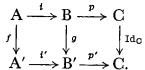
\includegraphics[keepaspectratio]{images/part002_08e8b4be.jpg}}

\begin{enumerate}
\def\labelenumi{(\roman{enumi})}
\setcounter{enumi}{3}
\tightlist
\item
  If \(b \in \mathbf{B}\) and \(a' \in \mathbf{A}'\) , then
\end{enumerate}

\[
g (b) i ^ {\prime} \left(a ^ {\prime}\right) g (b) ^ {- 1} = i ^ {\prime} (\omega (b) a ^ {\prime}).
\]

\begin{enumerate}
\def\labelenumi{(\roman{enumi})}
\tightlist
\item
  For \(a_{1}\) , \(a_{2}\) in A, we have, in B'',
\end{enumerate}

\[
\begin{array}{r l} (f (a _ {1} ^ {- 1}), i (a _ {1})) (f (a _ {2} ^ {- 1}), i (a _ {2})) & = (f (a _ {1} ^ {- 1}) (\omega (a _ {1}) f (a _ {2} ^ {- 1})), i (a _ {1}) i (a _ {2})) \\ & = (f (a _ {1} ^ {- 1}) f (a _ {1} a _ {2} ^ {- 1} a _ {1} ^ {- 1}), i (a _ {1} a _ {2})) \\ & = (f ((a _ {1} a _ {2}) ^ {- 1}, i (a _ {1} a _ {2})) \end{array}
\]

and hence \(a \mapsto (f(a^{-1}), i(a))\) is a homomorphism \(h\) of \(A\) into \(B''\) . Let \(a \in A\) , \(a' \in A'\) , \(b \in B\) ; then, in \(B''\) ,

\[
\begin{array}{r l} b h (a) b ^ {- 1} & = b f (a ^ {- 1}) a b ^ {- 1} = (\omega (b) f (a ^ {- 1})) (b a b ^ {- 1}) \\ & = f (b a ^ {- 1} b ^ {- 1}) (b a b ^ {- 1}) = h (b a b ^ {- 1}) \\ a ^ {\prime} h (a) a ^ {\prime - 1} & = a ^ {\prime} f (a ^ {- 1}) a a ^ {\prime - 1} = a ^ {\prime} f (a ^ {- 1}) (\omega (a) a ^ {\prime - 1}) a \\ & = a ^ {\prime} f (a ^ {- 1}) f (a) a ^ {\prime - 1} f (a ^ {- 1}) a = h (a) \end{array}
\]

and hence \(h(A) = D\) is normal in \(B''\) .

\begin{enumerate}
\def\labelenumi{(\roman{enumi})}
\setcounter{enumi}{1}
\tightlist
\item
  For \(a \in A\) ,
\end{enumerate}

\[
(p \circ q) (h (a)) = p (q (f (a ^ {- 1}) a)) = p (a) = e
\]

and hence \(p \circ q\) is trivial on D.

\begin{enumerate}
\def\labelenumi{(\roman{enumi})}
\setcounter{enumi}{2}
\tightlist
\item
  Let \(a' \in A'\) be such that \(i'(a') = e\) ; then \(a' \in D\) and hence there exists \(a \in A\) such that \(a' = f(a^{-1})a\) ; this implies \(a = e\) , whence \(a' = e\) ; thus \(i'\) is injective. As \(p\) and \(q\) are surjective, \(p'\) is surjective.
\end{enumerate}

Let \(r\) denote the canonical morphism of \(B''\) onto \(B'\) . Let \(a' \in A'\) , \(b \in B\) and \(b' = r(a'b)\) . If \(b' \in \operatorname{Im}(i')\) , there exists \(a_1' \in A'\) such that \(b' = r(a_1')\) ; then there exists \(a \in A\) such that \(a'b = a_1'f(a^{-1})a\) , whence \(b = a \in A\) and

\[
p ^ {\prime} (b ^ {\prime}) = p (q (a ^ {\prime} b)) = p (b) = e;
\]

thus, \(\operatorname{Im}(i') \subset \operatorname{Ker}(p')\) . We preserve the notation \(a', b, b'\) but assume that \(b' \in \operatorname{Ker}(p')\) ; then \(e = p'(b') = p(q(a'b)) = p(b)\) and hence \(b \in A\) , whence

\[
b ^ {\prime} = r (a ^ {\prime} f (b) f (b ^ {- 1}) b) = r (a ^ {\prime} f (b)) \in \operatorname{Im} (i ^ {\prime});
\]

thus \(\operatorname{Ker}(p') \subset \operatorname{Im}(i')\) .

If \(a\in \mathbf{A}\) , then

\[
i ^ {\prime} (f (a)) = r (f (a)) = r (f (a) f \left(a ^ {- 1}\right) a) = r (a) = g (i (a)).
\]

If \(b\in \mathbf{B}\) , then

\[
p ^ {\prime} (g (b)) = p (b)
\]

and hence diagram (4) is commutative.

\begin{enumerate}
\def\labelenumi{(\roman{enumi})}
\setcounter{enumi}{3}
\tightlist
\item
  Let \(b \in \mathbf{B}\) , \(a' \in \mathbf{A}'\) . Then
\end{enumerate}

\[
\begin{array}{r} g (b) i ^ {\prime} (a ^ {\prime}) g (b) ^ {- 1} = r (b) r (a ^ {\prime}) r (b) ^ {- 1} = r (b a ^ {\prime} b ^ {- 1}) \\ = r (\omega (b) a ^ {\prime}) = i ^ {\prime} (\omega (b) a ^ {\prime}). \end{array}
\]

PROPOSITION 20. Let G be a finite-dimensional real Lie group.

\begin{enumerate}
\def\labelenumi{(\roman{enumi})}
\item
  There exist a complex Lie group \(\tilde{\mathbf{G}}\) and an \(\mathbf{R}\) -analytic morphism \(\gamma\) of \(\mathbf{G}\) into \(\tilde{\mathbf{G}}\) with the following properties: for every complex Lie group \(\mathbf{H}\) and every \(\mathbf{R}\) -analytic morphism \(\phi\) of \(\mathbf{G}\) into \(\mathbf{H}\) , there exists one and only one \(\mathbf{C}\) -analytic morphism \(\psi\) of \(\tilde{\mathbf{G}}\) into \(\mathbf{H}\) such that \(\phi = \psi \circ \gamma\) .
\item
  If \((\tilde{\mathbf{G}}', \gamma')\) has the same properties as \((\tilde{\mathbf{G}}, \gamma)\) , there exists one and only one isomorphism \(\theta\) of \(\tilde{\mathbf{G}}\) onto \(\tilde{\mathbf{G}}'\) such that \(\theta \circ \gamma = \gamma'\) .
\item
  The \(\mathbf{C}\) -linear mapping of \(\mathrm{L}(\mathrm{G}) \otimes \mathbf{C}\) into \(\mathrm{L}(\tilde{\mathrm{G}})\) which extends \(\mathrm{L}(\gamma)\) is surjective; in particular \(\dim_{\mathbf{C}}(\tilde{\mathbf{G}}) \leqslant \dim_{\mathbf{R}}(\mathrm{G})\) .
\end{enumerate}

Assertion (ii) is obvious. We prove the existence of an ordered pair \((\tilde{G},\gamma)\) with properties (i) and (iii).

\begin{enumerate}
\def\labelenumi{(\alph{enumi})}
\tightlist
\item
  Suppose first that \(G\) is connected. Let \(g = L(G)\) , \(g_{\mathbf{C}} = g \otimes_{\mathbf{R}} \mathbf{C}\) be the complexification of \(g\) , \(S\) (resp. \(S'\) ) the simply connected real (resp. complex) Lie group with Lie algebra \(g\) (resp. \(g_{\mathbf{C}}\) ) and \(\sigma\) the unique \(\mathbf{R}\) -analytic morphism of \(S\) into \(S'\) such that \(L(\sigma)\) is the canonical injection of \(g\) into \(g_{\mathbf{C}}\) . Let \(\pi\) be the unique \(\mathbf{R}\) -analytic morphism of \(S\) onto \(G\) such that \(L(\pi) = I d_{L(G)}\) and \(F = K e r \pi\) .
\end{enumerate}

\pandocbounded{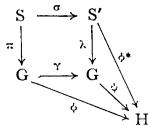
\includegraphics[keepaspectratio]{images/part002_6429af2f.jpg}}

For every complex Lie group H and every R-analytic morphism \(\phi\) of G into H, \(L(\phi): g \to L(H)\) has a unique C-linear extension to \(g_{C}\) and this extension is of the form \(L(\phi^{*})\) , where \(\phi^{*}\) is a C-analytic morphism of \(S'\) into H. Then

\[
\mathrm{L} (\phi \circ \pi) = \mathrm{L} (\phi) \circ \mathrm{L} (\pi) = \mathrm{L} (\phi) = \mathrm{L} (\phi^ {*}) \circ \mathrm{L} (\sigma) = \mathrm{L} (\phi^ {*} \circ \sigma)
\]

and hence \(\phi \circ \pi = \phi^{*} \circ \sigma\) . Therefore \(\phi^{*}(\sigma(F)) = \phi(\pi(F)) = \{e\}\) , whence

\[
\sigma (\mathrm{F}) \subset \operatorname{Ker} \phi^ {*}.
\]

Let P be the intersection of the Ker \(\phi^{*}\) for variable \(\phi\) . This is a normal Lie subgroup of \(S'\) (no. 2, Corollary 3 to Proposition 1). Let \(\tilde{G} = S'/P\) and \(\lambda: \mathbf{S}' \to \tilde{\mathbf{G}}\) be the canonical morphism. Then \(\sigma(\mathbf{F}) \subset \mathbf{P}\) and hence there exists one and only one \(\mathbf{R}\) -analytic morphism \(\gamma\) of \(\mathbf{G}\) into \(\tilde{\mathbf{G}}\) such that \(\gamma \circ \pi = \lambda \circ \sigma\) . If \(\psi: \tilde{\mathbf{G}} \to \mathbf{H}\) denotes the morphism derived from \(\phi^*\) when passing to the quotient, then

\[
(\phi \circ \gamma) \circ \pi = \psi \circ (\lambda \circ \sigma) = \phi^ {*} \circ \sigma = \phi \circ \pi
\]

whence \(\psi \circ \gamma = \phi\) . Clearly \(\mathrm{L}(\psi)\) , and hence \(\psi\) , are determined uniquely by the equality \(\psi \circ \gamma = \phi\) . Thus we have proved that the ordered pair \((\tilde{G}, \gamma)\) has properties (i) and (iii).

\begin{enumerate}
\def\labelenumi{(\alph{enumi})}
\setcounter{enumi}{1}
\tightlist
\item
  We pass now to the general case. Let \(\mathbf{F}\) be the identity component of \(\mathrm{G},\mathrm{M} = \mathrm{G} / \mathrm{F}\) and \(i\colon \mathrm{F}\to \mathrm{G}\) and \(p\colon \mathrm{G}\rightarrow \mathrm{M}\) be the canonical morphisms. We apply part (a) of the proof to F. We obtain an ordered pair \((\tilde{\mathbf{F}},\delta)\) . For all \(g\in \mathrm{G}\) , Int \(g|\mathrm{F} = \omega '(g)\) is an automorphism of F. By the universal property of \(\tilde{\mathbf{F}}\) , there exists one and only one automorphism \(\omega (g)\) of the complex Lie group \(\tilde{\mathbf{F}}\) such that \(\delta \circ \omega '(g) = \omega (g)\circ \delta\) . Clearly \(\omega\) is a morphism of G into \(\operatorname {Aut}(\tilde{\mathbf{F}})\) . If \(g\in \mathbf{G}\) and \(f\in \tilde{\mathbf{F}}\) , then
\end{enumerate}

\[
\delta (g f g ^ {- 1}) = (\delta \circ \omega^ {\prime} (g)) (f) = (\omega (g) \circ \delta) (f) = \omega (g) (\delta (f)).
\]

If \(f \in \mathbf{F}\) , then \(\delta \circ (\operatorname{Int}_{\mathbb{F}} f) = (\operatorname{Int}_{\tilde{\mathbb{F}}} \delta(f)) \circ \delta\) and \(\operatorname{Int}_{\tilde{\mathbb{F}}} \delta(f)\) is an automorphism of the complex Lie group \(\tilde{\mathbf{F}}\) ; hence \(\operatorname{Int}_{\tilde{\mathbb{F}}} \delta(f) = \omega(f)\) .

Hence Lemma 7 can be applied, which gives a diagram

\[
\begin{array}{c} \mathrm{F} \xrightarrow {i} \mathrm{G} \xrightarrow {p} \mathrm{M} \\ \delta \Big \downarrow \qquad \qquad \qquad \gamma \Big \downarrow \qquad \qquad \Big \downarrow \mathrm{Id} \\ \tilde {\mathrm{F}} \xrightarrow {\tilde {i}} \tilde {\mathrm{G}} \xrightarrow {\tilde {p}} \mathrm{M}. \end{array}
\]

Let \(\tilde{\mathbf{F}}\) be identified with a normal subgroup of \(\tilde{\mathbf{G}}\) by means of \(\tilde{i}\) . The group \(\tilde{\mathbf{G}}\) is generated by \(\tilde{\mathbf{F}}\) and \(\gamma (\mathbf{G})\) ; hence the automorphisms of \(\tilde{\mathbf{F}}\) defined by the elements of \(\tilde{\mathbf{G}}\) are automorphisms of the complex Lie group structure. By § 1, no. 9, Proposition 18, there exists one and only one complex Lie group structure on \(\tilde{\mathbf{G}}\) such that \(\tilde{\mathbf{F}}\) is an open Lie subgroup of \(\tilde{\mathbf{G}}\) . Henceforth \(\tilde{\mathbf{G}}\) will have this structure. As \(\delta\) is \(\mathbf{R}\) -analytic, \(\gamma\) is \(\mathbf{R}\) -analytic.

The ordered pair \((\tilde{G},\gamma)\) has property (iii) of the proposition. We show that it has property (i). Let H be a complex Lie group and \(\phi\) an R-analytic morphism of G into H. There exists a C-analytic morphism \(\eta\) of \(\tilde{F}\) into H such that \(\eta \circ \delta = \phi |F\) . Let \(g\in G\) . The mappings

\[
f \mapsto \eta (\omega (g) f), \quad f \mapsto \phi (g) \eta (f) \phi (g) ^ {- 1}
\]

of \(\tilde{\mathbf{F}}\) into \(\mathbf{H}\) are \(\mathbf{C}\) -analytic morphisms; they coincide on \(\delta(\mathbf{F})\) , for, if \(f' \in \mathbf{F}\) , then

\[
\begin{array}{r} \phi (g) \eta (\delta (f ^ {\prime})) \phi (g) ^ {- 1} = \phi (g) \phi (f ^ {\prime}) \phi (g) ^ {- 1} = \phi (g f ^ {\prime} g ^ {- 1}) \\ = \eta (\delta (g f ^ {\prime} g ^ {- 1})) = \eta (\omega (g) \delta (f ^ {\prime})); \end{array}
\]

therefore \(\eta (\omega (g)f) = \phi (g)\eta (f)\phi (g)^{-1}\) for all \(g\in G\) and all \(f\in \tilde{\mathbf{F}}\) . If \(\mathbf{G}'\) denotes the semi-direct product of \(\mathbf{G}\) by \(\tilde{\mathbf{F}}\) relative to \(\omega\) , there then exists a morphism \(\zeta\) of the group \(\mathbf{G}'\) into \(\mathrm{H}\) which coincides with \(\phi\) on \(\mathrm{G}\) and with \(\eta\) on \(\tilde{\mathbf{F}}\) . For \(f\in \mathbf{F}\) ,

\[
\zeta (\delta (f ^ {- 1}) f) = \eta (\delta (f ^ {- 1})) \phi (f) = \phi (f ^ {- 1}) \phi (f) = e.
\]

Hence \(\zeta\) defines on passing to the quotient a morphism \(\psi\) of \(\tilde{\mathbf{G}}\) into H. Then \(\psi \circ \gamma = \phi\) and \(\psi \circ \tilde{i} = \eta\) ; the latter equality implies that \(\psi\) is C-analytic.

Finally, let \(\psi'\) be a \(\mathbf{C}\) -analytic morphism of \(\tilde{\mathbf{G}}\) into \(\mathbf{H}\) such that \(\phi = \psi' \circ \gamma\) . Then

\[
\psi^ {\prime} \circ \tilde {i} \circ \delta = \psi^ {\prime} \circ \gamma \circ i = \phi \circ i = \psi \circ \tilde {i} \circ \delta
\]

and hence \(\psi' \circ \tilde{i} = \psi \circ \tilde{i}\) . As \(\tilde{G}\) is generated by \(\tilde{i}(\tilde{\mathrm{F}})\) and \(\gamma(G)\) , \(\psi' = \psi\) .

DEFINITION 4. \((\tilde{G},\gamma)\), or simply \(\tilde{G}\) , is called the universal complexification of G.

Remarks. (1) Let \((\tilde{\mathbf{G}},\gamma)\) be the universal complexification of G. Let \(G_0\) (resp. \(\tilde{G}_0\) ) be the identity component of G (resp. \(\tilde{G}\) ). By the proof of Proposition 20, \((\tilde{G}_0,\gamma |G_0)\) is the universal complexification of \(G_0\) and the composite morphism

\[
\mathrm{G} \rightarrow \tilde {\mathrm{G}} \rightarrow \tilde {\mathrm{G}} / \tilde {\mathrm{G}} _ {0}
\]

defines on passing to the quotient an isomorphism of \(\mathbf{G} / \mathbf{G}_0\) onto \(\tilde{\mathbf{G}} / \tilde{\mathbf{G}}_0\) .

\begin{enumerate}
\def\labelenumi{(\arabic{enumi})}
\setcounter{enumi}{1}
\tightlist
\item
  Suppose that G is simply connected. Let \(g = L(G)\) , \(g_{c}\) be the complexification of g, \(S'\) the simply connected complex Lie group with Lie algebra \(g_{c}\) and \(\sigma\) the morphism of G into \(S'\) such that \(L(\sigma)\) is the canonical injection of g into \(g_{c}\) . We again use the notation of the proof of Proposition 20, part (a). If \(H = S'\) and \(\phi = \sigma\) , then \(\phi^{*} = I d_{g}\) . Hence \((S', \sigma)\) is the universal complexification of G. Note that \(\sigma\) is not in general injective (Exercise 16); however its kernel is discrete since \(L(\sigma)\) is injective. On the other hand, let \(\theta\) be the involution of \(g_{c}\) defined by g and let \(\eta\) be the corresponding automorphism of the underlying real Lie group of \(S'\) ; let \(S'^{\eta}\) be the set of points of \(S'\) invariant under \(\eta\) ; it is a real Lie subgroup of \(S'\) with Lie algebra g (§3, no. 8, Corollary 1 to Proposition 29). By no. 1, Corollary 1 to Proposition 1, \(\sigma(G)\) is a real integral subgroup of \(S'\) with Lie algebra g and hence \(\sigma(G)\) is the identity component of \(S'^{\eta}\) ; in particular \(\sigma(G)\) is a real Lie subgroup of \(S'\) .
\end{enumerate}

\section{LIE GROUPS OVER AN ULTRAMETRIC FIELD}

In this paragraph, the valued field K is assumed to be ultrametric and of characteristic 0. Let A denote the valuation ring of K, m the maximal ideal of A and p the characteristic of the residue field A/m. If K is locally compact, then \(p \neq 0\) (Commutative Algebra, Chapter VI, § 9, Theorem 1).

\subsection{PASSAGE FROM LIE ALGEBRAS TO LIE GROUPS}

PROPOSITION 1. Let G be a Lie group germ with identity element e. There exists a fundamental system of open neighbourhoods of e in G consisting of Lie subgroups of G.

Let \(\mathrm{L}(\mathrm{G})\) be given a norm compatible with its topology and such that \(\| [x,y]\| \leqslant \| x\| \| y\|\) for all \(x,y\) in \(\mathrm{L}(\mathrm{G})\) . Let \(\mathrm{G}_1\) be the Lie group defined by \(\mathrm{L}(\mathrm{G})\) . By § 4, no. 2, Theorem 2, G and \(\mathrm{G}_1\) are locally isomorphic. Then it suffices to apply § 4, no. 2, Lemma 3 (iii).

THEOREM 1. Let \(\mathbf{L}\) be a complete normable Lie algebra. There exists a Lie group \(\mathbf{G}\) such that \(\mathbf{L}(\mathbf{G})\) is isomorphic to \(\mathbf{L}\) . Two such groups are locally isomorphic.

The first assertion has been proved in § 4, no. 2, Lemma 3. The second is a special case of § 4, no. 2, Theorem 2.

THEOREM 2. Let G be a Lie group and b a Lie subalgebra of L(G) admitting a topological supplement. There exists a Lie subgroup H of G such that L(H) = b. If H₁ and H₂ are Lie subgroups of G such that L(H₁) = L(H₂) = b, then H₁ ∩ H₂ is open in H₁ and H₂.

The first assertion follows from Proposition 1 and §4, no. 2, Theorem 3. The second is a special case of §4, no. 2, Theorem 3.

THEOREM 3. Let \(\mathbf{G}\) and \(\mathbf{H}\) be Lie groups and \(h\) a continuous morphism of \(\mathbf{L}(\mathbf{G})\) into \(\mathbf{L}(\mathbf{H})\) .

\begin{enumerate}
\def\labelenumi{(\roman{enumi})}
\item
  There exist an open subgroup \(\mathbf{G}'\) of \(\mathbf{G}\) and a Lie group morphism \(\phi\) of \(\mathbf{G}'\) into \(\mathbf{H}\) such that \(h = \mathbf{L}(\phi)\) .
\item
  Let \(\mathbf{G}_1, \mathbf{G}_2\) be open subgroups of \(\mathbf{G}\) and \(\phi_i\) a morphism of \(\mathbf{G}_i\) into \(\mathbf{H}\) such that \(h = \mathbf{L}(\phi_i)\) . Then \(\phi_1\) and \(\phi_2\) coincide on an open subgroup of \(\mathbf{G}\) .
\end{enumerate}

By Proposition 1, this follows from § 4, no. 1, Theorem 1.

PROPOSITION 2. Let \(\mathbf{G}\) be a Lie group and \(\mathfrak{h}\) a Lie subalgebra of \(\mathbf{L}(\mathbf{G})\) admitting a topological supplement. The following conditions are equivalent:

\begin{enumerate}
\def\labelenumi{(\roman{enumi})}
\item
  There exist an open subgroup \(\mathbf{G}'\) of \(\mathbf{G}\) and a normal Lie subgroup \(\mathbf{H}\) of \(\mathbf{G}'\) such that \(\mathrm{L(H)} = \mathfrak{h}\) .
\item
  \(\mathfrak{h}\) is an ideal of \(\mathrm{L}(\mathrm{G})\) .
\end{enumerate}

If there exist \(G'\) and \(H\) with the properties of (i), then \(L(G') = L(G)\) and \(L(H)\) is an ideal of \(L(G')\) by § 3, no. 12, Proposition 47.

Suppose that \(\mathfrak{h}\) is an ideal of \(\mathrm{L}(\mathrm{G})\) . There exists a Lie group \(\mathrm{F}\) such that \(\mathrm{L}(\mathrm{F}) = \mathrm{L}(\mathrm{G}) / \mathfrak{h}\) (Theorem 1). Let \(h\) be the canonical morphism of \(\mathrm{L}(\mathrm{G})\) onto \(\mathrm{L}(\mathrm{F})\) . By Theorem 3 (i), there exist an open subgroup \(\mathrm{G}'\) of \(\mathrm{G}\) and a Lie group morphism \(\phi\) of \(\mathrm{G}'\) into \(\mathrm{F}\) such that \(\mathrm{L}(\phi) = \mathrm{h}\) . By § 3, no. 8, the kernel \(\mathrm{H}\) of \(\phi\) is a Lie subgroup of \(\mathrm{G}'\) and \(\mathrm{L}(\mathrm{H}) = \mathrm{Ker} \, \mathrm{L}(\phi) = \mathrm{Ker} \, h = \mathfrak{h}\) . Finally, \(\mathrm{H}\) is normal in \(\mathrm{G}'\) since \(\mathrm{H} = \mathrm{Ker} \, \phi\) .

\subsection{EXPONENTIAL MAPPINGS}

PROPOSITION 3. Let \(\mathbf{G}\) be a Lie group. There exists an exponential mapping \(\phi\) of \(\mathbf{G}\) with the following properties:

\begin{enumerate}
\def\labelenumi{(\roman{enumi})}
\item
  \(\phi\) is defined on an open subgroup U of the additive group L(G);
\item
  \(\phi (\mathbf{U})\) is an open subgroup of \(\mathbf{G}\) and \(\phi\) is an isomorphism of the analytic manifold \(\mathbf{U}\) onto the analytic manifold \(\phi (\mathbf{U})\) ;
\item
  \(\phi(nx) = \phi(x)^n\) for all \(x \in \mathbf{U}\) and all \(n \in \mathbf{Z}\) .
\end{enumerate}

Let \(\dot{\mathrm{L}}(\mathrm{G})\) be given a norm compatible with its topology and such that \(\| [x,y]\| \leqslant \| x\| \| y\|\) for \(x,y\) in \(\mathrm{L}(\mathrm{G})\) . Let \(\mathbf{G}_1\) be the Lie group defined by \(\mathrm{L}(\mathrm{G})\) . Let \(\psi = \mathrm{Id}_{\mathrm{G}_1}\) , which is an exponential mapping of \(\mathbf{G}_1\) . For all \(\mu >0\) , let \(\mathrm{L}_{\mu}\) be the set of \(x\in \mathrm{L}(\mathrm{G})\) such that \(\| x\| < \mu\) . Then, for \(\mu\) sufficiently small, \(\mathrm{L}_{\mu}\) is an open subgroup of the additive group \(\mathrm{L}(\mathrm{G}),\psi (\mathrm{L}_{\mu})\) is an open subgroup of \(\mathrm{G}_1\) (§ 4, no. 2, Lemma 3), \(\psi |\mathrm{L}_{\mu}\) is an isomorphism of analytic manifolds of \(\mathrm{L}_{\mu}\) onto \(\psi (\mathrm{L}_{\mu})\) and \(\psi (nx) = \psi (x)^n\) for all \(x\in \mathrm{L}_{\mu}\) and all \(n\in \mathbf{Z}\) . The \(\mathrm{L}_{\mu}\) form a fundamental system of neighbourhoods of 0 in \(\mathrm{L}(\mathrm{G})\) . By Theorem 1, there exist \(\mu\) and an open subgroup \(\mathbf{G}'\) of \(\mathbf{G}\) such that \(\psi (\mathrm{L}_{\mu})\) and \(\mathbf{G}'\) are isomorphic, whence the proposition.

PROPOSITION 4. Let G be a Lie group and \(\phi\) an injective exponential mapping of G. Suppose that \(p > 0\) . For all \(x, y\) in L(G),

\begin{enumerate}
\def\labelenumi{(\arabic{enumi})}
\tightlist
\item
\end{enumerate}

\[
x + y = \lim _ {n \rightarrow + \infty} p ^ {- n} \phi^ {- 1} (\phi (p ^ {n} x) \phi (p ^ {n} y))\tag{1}
\]

\[
[ x, y ] = \lim _ {n \rightarrow + \infty} p ^ {- 2 n} \phi^ {- 1} (\phi (p ^ {n} x) \phi (p ^ {n} y) \phi (- p ^ {n} x) \phi (- p ^ {n} y)).\tag{2}
\]

These are special cases of Proposition 4 of § 4, no. 3.

\subsection{STANDARD GROUPS†}

If \(\mathrm{S}(\mathbf{X}_{1},\mathbf{X}_{2},\ldots,\mathbf{X}_{n})\) is a formal power series with coefficients in A, then, for all \(x_{1},\ldots,x_{r}\) in m, the series \(\mathrm{S}(x_{1},x_{2},\ldots,x_{r})\) is convergent. More precisely, \(m\times m\times\cdots\times m\) is contained in the domain of absolute convergence of S (Differentiable and Analytic Manifolds, R, 4.1.3).

DEFINITION 1. Let \(r\) be an integer \(\geqslant 0\) . A standard group of dimension \(r\) over \(\mathbf{K}\) is a Lie group \(G\) with the following properties:

\begin{enumerate}
\def\labelenumi{(\roman{enumi})}
\item
  the underlying analytic manifold of G is m × m × · · · × m (r factors);
\item
  there exists a formal power series \(\mathbf{F}\) in \(2r\) variables with coefficients in \(\mathbf{A}^r\) , without constant term, such that \(x.y = \mathbf{F}(x,y)\) for all \(x,y\) in \(\mathbf{G}\) .
\end{enumerate}

Then 0.0 = 0 and hence the identity element of G is the origin of m × m · · · × m.
† The results of nos. 3 and 4 and their proofs remain true when the characteristic of K is > 0.

L(G) will be identified with \(K^r\). By § 5, formula (13), the constants of structure of L(G) with respect to the canonical basis belong to A. We shall need, in the same proof to consider the elements of m × ⋯ × m, now as elements of G, now as elements of L(G).

Example. Let \(G = 1 + \mathbf{M}_{n}(m)\) , which is an open subset of \(\mathbf{M}_{n}(\mathbf{K})\) . If \(x \in G\) , then det \(x \in 1 + m\) and hence \(G \subset \mathbf{GL}(n, K)\) . Clearly \(GG \subset G\) . If \(x = 1 + y\) with \(y \in \mathbf{M}_{n}(m)\) , the calculation of the inverse of a matrix proves first that \(x^{-1} \in \mathbf{M}_{n}(\mathbf{A})\) ; if we write \(x^{-1} = 1 + y'\) , then \(y + y' + yy' = 0\) , hence \(y' \in \mathbf{M}_{n}(m)\) and therefore \(x^{-1} \in G\) . Thus G is an open subgroup of \(\mathbf{GL}(n, K)\) . We identify G with \(m^{n^2}\) by means of the mapping \((\delta_{ij} + y_{ij}) \mapsto (y_{ij})\) . Clearly G is a standard group.

THEOREM 4. Let G be a finite-dimensional Lie group. There exists an open subgroup of G isomorphic to a standard group.

By replacing G by a group isomorphic to an open subgroup of G, the problem is reduced to the case where G is an open subset of \(K^{r}\) , with identity element 0 and where the coordinates of the product x.y and the inverse \(x^{[-1]}\) are given by formulae

\begin{enumerate}
\def\labelenumi{(\arabic{enumi})}
\setcounter{enumi}{2}
\tightlist
\item
\end{enumerate}

\[
(x. y) _ {i} = x _ {i} + y _ {i} + \sum_ {| \alpha | \geqslant 1, | \beta | \geqslant 1} c _ {\alpha \beta i} x ^ {\alpha} y ^ {\beta} (i = 1, 2, \dots , r)\tag{3}
\]

\[
(x ^ {[ - 1 ]}) _ {i} = - x _ {i} + \sum_ {| \alpha | > 1} d _ {\alpha i} x ^ {\alpha} \quad (i = 1, 2, \dots , r)\tag{4}
\]

where the series on the right hand side are convergent for \(x, y\) in \(G\) (§ 5, no. 1). Let \(\lambda \in K^*\) and let the group law be transported from \(G\) to \(G' = \lambda G\) by the homothety of ratio \(\lambda\) . For \(x', y'\) in \(G'\) , the product \(x'.y'\) and the inverse \(x'^{(-1)}\) evaluated in \(G'\) have coordinates

\[
(x ^ {\prime}. y ^ {\prime}) _ {i} = x _ {i} ^ {\prime} + y _ {i} ^ {\prime} + \sum_ {| \alpha | \geqslant 1, | \beta | \geqslant 1} c _ {\alpha \beta i} ^ {\prime} x ^ {\prime \alpha} y ^ {\prime \beta} (i = 1, 2, \dots , r)
\]

\[
(x ^ {\prime [ - 1 ]}) _ {i} = - x _ {i} ^ {\prime} + \sum_ {| \alpha | > 1} d _ {\alpha i} ^ {\prime} x ^ {\prime \alpha} \quad (i = 1, 2, \dots , r)
\]

where

\[
c _ {\alpha \beta i} ^ {\prime} = \lambda^ {- | \alpha | - | \beta | + 1} c _ {\alpha \beta i}, \quad d _ {\alpha i} ^ {\prime} = \lambda^ {- | \alpha | + 1} d _ {\alpha i}.
\]

As the series (3) and (4) are convergent, we see that, for \(|\lambda|\) sufficiently large, for all \(\alpha, \beta, i\) ,

\[
\left| c _ {\alpha \beta i} ^ {\prime} \right| \leqslant 1, \quad \left| d _ {\alpha i} ^ {\prime} \right| \leqslant 1
\]

that is \(c_{\alpha\beta i}^{\prime}\in A\) and \(d_{\alpha i}^{\prime}\in A\) ; and on the other hand \(G^{\prime}\supset m\times m\times\cdots\times m\) . Then \(m\times m\times\cdots\times m\) is an open subgroup of \(G^{\prime}\) and is a standard group.

\subsection{FILTRATION OF STANDARD GROUPS}

We again use the notation of Definition 1. We choose a number \(a > 1\) and a real valuation \(v\) of \(\mathbf{K}\) such that \(|x| = a^{-v(x)}\) for all \(x \in \mathbf{K}\) (Commutative Algebra, Chapter VI, §6, Proposition 3). If \(a\) is a non-zero (and hence open) ideal of A contained in m, let \(\mathrm{G}(a)\) denote the set of elements of G whose coordinates belong to \(a\) . If \(\lambda \in \mathbf{R}\) , let \(a_{\lambda}\) (resp. \(a_{\lambda}^{+}\) ) denote the set of \(x \in \mathbf{K}\) such that \(v(x) \geqslant \lambda\) (resp. \(v(x) > \lambda\) ); then \(a_0 = A\) , \(a_0^+ = m\) . For \(x = (x_1, \ldots, x_r) \in G\) , we shall write

\[
\omega (x) = \inf (v (x _ {1}), \dots , v (x _ {r})).\tag{5}
\]

PROPOSITION 5. Let G be a standard group.

\begin{enumerate}
\def\labelenumi{(\roman{enumi})}
\item
  If \(\mathfrak{a}\) is a non-zero ideal of \(\mathbf{A}\) contained in \(\mathfrak{m}\) , \(\mathbf{G}(\mathfrak{a})\) is an open normal subgroup of \(\mathbf{G}\) .
\item
  The \(\mathbf{G}(\mathfrak{a}_{\lambda})\) , for \(\lambda > 0\) , form a fundamental system of neighbourhoods of \(e\) in \(\mathbf{G}\) .
\item
  Suppose that \(\mathfrak{a}_{\lambda} \subset \mathfrak{a}\) for \(\lambda \geqslant \lambda_0\) and let the \(G(\mathfrak{a}) / G(\mathfrak{a}_{\lambda})\) , for \(\lambda \geqslant \lambda_0\) , be given the discrete topology. Then the topological group \(G(\mathfrak{a})\) is the inverse limit of the groups \(G(\mathfrak{a}) / G(\mathfrak{a}_{\lambda})\) .
\item
  Let \(\mathfrak{a},\mathfrak{b}\) be non-zero ideals of A contained in \(\mathfrak{m}\) such that \(\mathfrak{a} \supset \mathfrak{b} \supset \mathfrak{a}^2\) . The mapping \(x \mapsto (x_1 \bmod \mathfrak{b}, \ldots, x_r \bmod \mathfrak{b})\) of G(a) into (a/b) × · · · × (a/b) defines on passing to the quotient an isomorphism of the group G(a)/G(b) onto the additive group (a/b) × · · · × (a/b).
\end{enumerate}

If \(x \in G\) and \(y \in G(a)\) , the coordinates of \(x\) and \(x.y\) are equal modulo \(a\) . Hence, for \(x'\) , \(x''\) in \(G\) and \(y'\) , \(y''\) in \(G(a)\) , the coordinates of \(x'.x''\) and \((x'.y')\) . \((x''.y'')\) are equal modulo \(a\) . This proves (i).

\begin{enumerate}
\def\labelenumi{(\roman{enumi})}
\setcounter{enumi}{1}
\item
  is obvious.
\item
  follows from the above and General Topology, Chapter III, § 7, Proposition 2.
\end{enumerate}

If \(x \in G(a)\) and \(y \in G(a)\) , the coordinates of \(x, y\) are congruent to those of \(x + y\) modulo \(G(a^2)\) by formula (4) of § 5. This proves (iv).

COROLLARY. Suppose that K is locally compact and let \(q = \operatorname{Card}(\mathbf{A} / \mathfrak{m})\) .

\begin{enumerate}
\def\labelenumi{(\roman{enumi})}
\item
  If \(a = m^{a}\) and \(b = m^{b}\) with \(b \geqslant a \geqslant 1\) , \(\mathrm{G}(a)/\mathrm{G}(b)\) is a p-group of cardinal \(q^{r(b-a)}\) .
\item
  G(a) is an inverse limit of p-groups.
\end{enumerate}

The number of elements in \(\mathrm{G}(\mathfrak{a})/\mathrm{G}(\mathfrak{b})\) is \((\mathrm{Card}(\mathfrak{a}/\mathfrak{b}))^{r}\) ; if \(b=a+1\) , a/b is a 1-dimensional vector space over A/m, whence (i) in this case; the general case follows by induction on b-a. Assertion (ii) follows from (i) and Proposition 5 (iii).

PROPOSITION 6. Let \(\mathfrak{a}, \mathfrak{b}, \mathfrak{c}, \mathfrak{c}'\) be non-zero ideals of \(\mathbf{A}\) contained in \(\mathfrak{m}\) such that

\[
\mathfrak {c} ^ {\prime} \subset \mathfrak {c}, \quad \mathfrak {a b} \subset \mathfrak {c}, \quad \mathfrak {a b} ^ {2} \subset \mathfrak {c} ^ {\prime}, \quad \mathfrak {a} ^ {2} \mathfrak {b} \subset \mathfrak {c} ^ {\prime}.
\]

If \(x \in \mathrm{G}(\mathfrak{a})\) and \(y \in \mathrm{G}(\mathfrak{b})\) , then \(x^{[-1]}y^{[-1]}x.y, x.y.x^{[-1]}y^{[-1]}\) and \([x,y]\) belong to \(\mathrm{G}(\mathfrak{c})\) and are congruent modulo \(\mathrm{G}(\mathfrak{c}')\) .

By § 5, no. 2, Proposition 1, there exist \(c_{\alpha \beta} \in \mathbf{A}^r\) such that

\[
x ^ {[ - 1 ]}. y ^ {[ - 1 ]}. x. y - [ x, y ] = \sum_ {| \alpha | + | \beta | \geqslant 3} c _ {\alpha \beta} x ^ {\alpha} y ^ {\beta}.
\]

If \(x = 0\) or \(y = 0\) , then \(x^{[-1]}y^{[-1]}x.y - [x,y] = 0\) ; hence \(c_{0\beta} = c_{\alpha 0} = 0\) . On the other hand, the conditions

\[
x \in \mathrm{G} (\mathfrak {a}), \quad y \in \mathrm{G} (\mathfrak {b}), \quad | \alpha | \geqslant 1, \quad | \beta | \geqslant 1, \quad | \alpha | + | \beta | \geqslant 3
\]

imply

\[
c _ {\alpha \beta} x ^ {\alpha} y ^ {\beta} \in \mathrm{G} (a ^ {2} b + a b ^ {2}) \subset \mathrm{G} (c ^ {\prime})
\]

and hence \(x^{[-1]} \cdot y^{[-1]}x \cdot y - [x, y] \in \mathrm{G}(\mathfrak{c}')\) . We see similarly that

\[
x. y. x ^ {[ - 1 ]}. y ^ {[ - 1 ]} - [ x, y ] \in \mathrm{G} (\mathfrak {c} ^ {\prime}).
\]

Finally, by § 5, formula (13), \([x,y] \in G(\mathfrak{ab}) \subset G(\mathfrak{c})\) .

PROPOSITION 7. (i) The family \((\mathrm{G}(\mathfrak{a}_{\lambda}))\) is a central filtration on \(\mathbf{G}\) (Chapter II, § 4, no. 4, Definition 2).

\[
\text { (ii) } For \lambda \in \mathbf {R} _ {+} ^ {*}, G (a _ {\lambda}) = \{x \in G | \omega (x) \geqslant \lambda \}, G (a _ {\lambda} ^ {+}) = \{x \in G | \omega (x) > \lambda \}.
\]

\begin{enumerate}
\def\labelenumi{(\roman{enumi})}
\setcounter{enumi}{1}
\tightlist
\item
  is obvious. We prove (i). Clearly \(G(a_{\lambda}) = \bigcap_{\mu < \lambda} G(a_{\mu})\) and \(G = \bigcup_{\lambda > 0} G(a_{\lambda})\) . On the other hand, if \(x \in G(a_{\lambda})\) and \(y \in G(a_{\mu})\) , then
\end{enumerate}

\[
x ^ {[ - 1 ]}. y ^ {[ - 1 ]}. x. y \in G (a _ {\lambda + \mu})
\]

by Proposition 6 applied with \(a = a_{\lambda}, b = a_{\mu}, c = c' = a_{\lambda + \mu}\) .

By Chapter II, § 4, no. 4, we can form the group gr(G) associated with the group G, with the central filtration \((G(a_\lambda))\). Writing \(G_\lambda = G(a_\lambda)/G(a_\lambda^+)\) for all \(\lambda > 0\), we obtain \(gr(G) = \bigoplus_{\lambda>0} G_\lambda\). Recall (loc. cit., Proposition 1) that the commutator in G allows us to define a bracket in gr(G) with which gr(G) is a Lie algebra, as follows: if \(x \in G_\lambda\) and \(y \in G_\mu\), choose a representative x of \(\bar{x}\) in \(G(a_\lambda)\) and a representative y of \(\bar{y}\) in \(G(a_\mu)\); then \([\bar{x},\bar{y}]\) is the class of \(x^{[-1]}.y^{[-1]}.x.y \in G(a_{\lambda+\mu})\) in \(G_{\lambda+\mu}\). By Proposition 6, applied with \(a = a_\lambda, b = a_\mu, c = a_{\lambda+\mu}, c' = a_{\lambda+\mu}\), we see that \([\bar{x},\bar{y}]\) is also the class of \([x,y]\) in \(G_{\lambda+\mu}\). Thus, when G is considered as a Lie subalgebra of L(G) = \(K^r\), filtered by the \(G(a_\lambda)\), the associated graded Lie algebra (Chapter II, § 4, no. 3) is equal to gr(G).

\subsection{POWERS IN STANDARD GROUPS}

We preserve the notation of no. 4.

PROPOSITION 8. Let \(n \in \mathbf{Z}\) and \(h_n\) be the mapping \(x \mapsto x^n\) of \(G\) into \(G\) . Let \(a\) be a non-zero ideal of \(A\) contained in \(m\) , such that \(n \notin a\) . Then \(h_n|G(a)\) is an isomorphism of the analytic manifold \(G(a)\) onto the analytic manifold \(G(na)\) .

By definition of standard groups, \(h_n\) is equal on the whole of \(G\) to the sum of an integral series with coefficients in \(A^r\) . By § 5, formula (4), this series is of the form

\[
h _ {n} (x) = n x + \sum_ {| \alpha | \geqslant 2} a _ {\alpha} x ^ {\alpha}.
\]

Hence, for \(x \in G\) ,

\[
\begin{array}{r l} h _ {n} (n x) & = n ^ {2} \Big (x + \sum_ {| \alpha | \geqslant 2} a _ {\alpha} n ^ {| \alpha | - 2} x ^ {\alpha} \Big) \\ & = n ^ {2} \mathrm{S} (x) \end{array}
\]

where we write \(\mathrm{S}(x)=x+\sum_{|\alpha| \geq 2} a_{\alpha} n^{|\alpha|-2} x^{\alpha}\) . This series \(\mathrm{S}(x)\) defines an analytic mapping, also denoted by S, of G into G. By Algebra, Chapter IV, §6, Proposition 8, there exists an integral series \(S'\) in r variables with coefficients in \(A^r\) such that \(\mathrm{S}'(\mathrm{S}(\mathrm{X}))=\mathrm{S}(\mathrm{S}'(\mathrm{X}))=\mathrm{X}\) . Hence S is an isomorphism of the analytic manifold G onto itself and, for every non-zero ideal b of A contained in m, \(\mathrm{S}(\mathrm{G}(\mathrm{b}))\subset\mathrm{G}(\mathrm{b}),\mathrm{S}'(\mathrm{G}(\mathrm{b}))\subset\mathrm{G}(\mathrm{b})\) and therefore

\[
\mathrm{S} (\mathrm{G} (\mathfrak {b})) = \mathrm{G} (\mathfrak {b}).
\]

As \(h_n(y) = n^2\mathrm{S}\left(\frac{1}{n} y\right)\) for \(y \in n\mathrm{G}\) , we see that \(h_n|n\mathrm{G}(\mathfrak{b})\) is an isomorphism of the analytic manifold \(n\mathrm{G}(\mathfrak{b})\) onto the analytic manifold \(n^2\mathrm{G}(\mathfrak{b})\) . But, as \(n \notin \mathfrak{a}\) , \(|n| > |\lambda|\) for all \(\lambda \in \mathfrak{a}\) , hence \(n^{-1}\mathfrak{a} \subset \mathfrak{m}\) and hence \(\mathfrak{a}\) is of the form \(n\mathfrak{b}\) where \(\mathfrak{b}\) is a non-zero ideal of \(\mathrm{A}\) contained in \(\mathfrak{m}\) .

COROLLARY. If \(n\) is invertible in A, \(h_n\) is an isomorphism of the analytic manifold G onto itself. For every non-zero ideal \(\mathfrak{a}\) of A contained in \(\mathfrak{m}\) , \(h_n(\mathrm{G}(\mathfrak{a})) = \mathrm{G}(\mathfrak{a})\) . For all \(x \in \mathrm{G}\) , \(\omega(x^n) = \omega(x)\) .

This follows immediately from Proposition 8.

PROPOSITION 9. Suppose that \(p \neq 0\) .

\begin{enumerate}
\def\labelenumi{(\roman{enumi})}
\item
  Let \(\mathfrak{a},\mathfrak{b}\) be non-zero ideals of \(\mathbf{A}\) such that \(\mathfrak{b} \subset \mathfrak{a} \subset \mathfrak{m}\) . In the group \(\mathrm{G}(\mathfrak{a}) / \mathrm{G}(\mathfrak{b})\) , every element has order a power of \(p\) .
\item
  Suppose that \(v(p) = 1\) . If \(x \in G\) is such that \(\omega(x) > \frac{1}{p - 1}\) , then
\end{enumerate}

\[
\omega (x ^ {p}) = \omega (x) + 1.
\]

By § 5, formula (4), for all \(x \in G\) ,

\[
x ^ {p} = p x + \sum_ {| \alpha | \geqslant 2} c _ {\alpha} x ^ {\alpha}
\]

where \(c_{\alpha} \in A^{r}\) for all \(\alpha\) . Even for proving (i) it can be assumed that \(v(p) = 1\) . Then if \(\omega(x) \geqslant 1\) , it follows that \(\omega(x^{p}) \geqslant \omega(x) + 1\) and hence \(\omega(x^{p^{n}})\) tends to \(+\infty\) as \(n\) tends to \(+\infty\) ; this proves (i). As \(\binom{p}{i}\) is divisible by \(p\) for

\(1 \leqslant i \leqslant p - 1\) , Proposition 2 of § 5, no. 3, proves that \(c_{\alpha} \in pA^{r}\) for

\[
2 \leqslant | \alpha | \leqslant p - 1
\]

and hence

\[
\omega \left(c _ {\alpha} x ^ {\alpha}\right) > \omega (p x) = \omega (x) + 1 \quad \text { for } 2 \leqslant | \alpha | \leqslant p - 1.
\]

On the other hand, if \(|\alpha| \geqslant p\) , \(\omega(c_{\alpha}x^{\alpha}) \geqslant p\omega(x)\) and \(p\omega(x) > \omega(x) + 1\) if \(\omega(x) > \frac{1}{p - 1}\) . This proves (ii).

\subsection{LOGARITHMIC MAPPING}

Lemma 1. Suppose that \(p \neq 0\) . Let \(G\) be a Lie group, \(G_1\) an open subgroup of \(G\) which is isomorphic to a standard group and \(x \in G\) . The following conditions are equivalent:

\begin{enumerate}
\def\labelenumi{(\roman{enumi})}
\item
  there exists a power of \(x\) which belongs to \(\mathbf{G}_1\) ;
\item
  there exists a strictly increasing sequence \((n_{i})\) of integers such that \(x^{n_{i}}\) tends to \(e\) as \(i\) tends to \(+\infty\) .
  (ii) \(\Rightarrow\) (i): obvious.
  (i) \(\Rightarrow\) (ii): suppose that \(y = x^{m} \in G_{1}\) . By Proposition 9 (i) of no. 5, \(y^{p^n}\) tends to \(e\) as \(n\) tends to \(+\infty\) , in other words \(x^{mp^n}\) tends to \(e\) as \(n\) tends to \(+\infty\) .
\end{enumerate}

PROPOSITION 10. Suppose that \(p \neq 0\) . Let \(G\) be a finite-dimensional Lie group. Let \(G_f\) be the set of \(x \in G\) for which there exists a strictly increasing sequence \((n_i)\) of integers such that \(x^{n_i}\) tends to \(e\) as \(i\) tends to \(+\infty\) .

\begin{enumerate}
\def\labelenumi{(\roman{enumi})}
\item
  \(G_{f}\) is open in G.
\item
  There exists one and only one mapping \(\psi\) of \(G_{f}\) into L(G) with the following properties:
\end{enumerate}

\begin{enumerate}
\def\labelenumi{(\alph{enumi})}
\item
  \(\psi (x^n) = n\psi (x)\) for all \(x\in \mathbf{G}_f\) and all \(n\in \mathbf{Z}\) ;
\item
  there exists an open neighbourhood \(\mathbf{V}\) of \(e\) in \(\mathbf{G}\) such that \(\psi |\mathbf{V}\) is the inverse mapping of an injective exponential mapping.
\end{enumerate}

\begin{enumerate}
\def\labelenumi{(\roman{enumi})}
\setcounter{enumi}{2}
\tightlist
\item
  The mapping \(\psi\) is analytic.
\end{enumerate}

There exists an open subgroup of \(\mathbf{G}\) which is isomorphic to a standard group (no. 3, Theorem 4). Assertion (i) then follows from Lemma 1.

Let U be an open subgroup of L(G) and \(\phi\colon\mathrm{U}\to\phi(\mathrm{U})\) an exponential mapping of G with the properties of Proposition 3 of no. 2. U can be assumed to be small enough for \(\phi(\mathrm{U})\subset\mathrm{G}_{f}\) . Let \(x\in\mathrm{G}_{f}\) . There exists \(m\in\mathbf{Z}-\{0\}\) such that \(x^{m}\in\phi(\mathrm{U})\) . The element \(\frac{1}{m}\phi^{-1}(x^{m})\) does not depend on the choice of \(m\) . For let \(m'\in\mathbf{Z}\) be such that \(x^{m'}\in\phi(\mathrm{U})\) . Then \(x^{mm'}\in\phi(\mathrm{U})\) and

\[
m ^ {\prime} \phi^ {- 1} (x ^ {m}) = \phi^ {- 1} (x ^ {m m ^ {\prime}}) = m \phi^ {- 1} (x ^ {m ^ {\prime}}),
\]

whence our assertion. Let \(\psi(x) = \frac{1}{m}\phi^{-1}(x^m)\) . Then \(\psi|\phi(U) = \phi^{-1}\) . On the other hand, if \(n \in \mathbf{Z}\) , then

\[
\psi (x ^ {n}) = \frac {1}{m} \phi^ {- 1} (x ^ {n m}) = \frac {n}{m} \phi^ {- 1} (x ^ {m}) = n \psi (x).
\]

Hence \(\psi\) has properties (a) and (b) of the proposition. In a neighbourhood of \(x\) , \(\psi\) is composed of the mappings \(x \mapsto x^m\) , \(y \mapsto \phi^{-1}(y)\) and \(z \mapsto \frac{1}{m} z\) ; hence \(\psi\) is analytic on \(G_f\) .

Finally, let \(\psi'\) be a mapping of \(G_f\) into L(G) and V' a neighbourhood of \(e\) in \(G_f\) such that \(\psi'(x^n) = n\psi'(x)\) for \(x \in G_f\) and \(n \in \mathbf{Z}\) and such that \(\psi'|V'\) is the inverse mapping of an injective exponential mapping. Then \(\psi\) and \(\psi'\) coincide on a neighbourhood W of \(e\) . If \(x \in G_f\) , there exists \(n \in \mathbf{Z}\) such that \(x^n \in W\) . Then

\[
n \psi^ {\prime} (x) = \psi^ {\prime} (x ^ {n}) = \psi (x ^ {n}) = n \psi (x)
\]

and hence \(\psi = \psi'\) .

DEFINITION 2. The mapping \(\psi\) of Proposition 10 is called the logarithmic mapping of G and is denoted by \(\log_{\mathbb{G}}\) or simply log.

PROPOSITION 11. Suppose that \(p \neq 0\) . Let \(x, y\) be two permutable elements of \(G_f\) . Then \(xy \in G_f\) and \(\log(xy) = \log x + \log y\) .

The fact that \(xy \in G_f\) follows from Lemma 1. Let \(U\) be an open subgroup of the additive group \(L(G)\) and \(\phi: U \to \phi(U)\) an exponential mapping of \(G\) with the properties of Proposition 3 of no. 2; \(U\) can be assumed to be small enough for \(\log(\phi(U))\) to be the inverse mapping of \(\phi\) . For \(n \in \mathbf{Z} - \{0\}\) suitably chosen, \(x^n \in \phi(U)\) , \(y^n \in \phi(U)\) . Let \(u = \log x^n\) , \(v = \log y^n\) , whence \(x^n = \phi(u)\) , \(y^n = \phi(v)\) . By formula (2), \([u,v] = 0\) . The Hausdorff formula proves then that \(\phi(\lambda(u + v)) = \phi(\lambda u)\phi(\lambda v)\) for \(|\lambda|\) sufficiently small; hence, for every sufficiently large integer \(i\) ,

\[
\phi (p ^ {i} (u + v)) = \phi (p ^ {i} u) \phi (p ^ {i} v)
\]

that is

\[
p ^ {i} (\log x ^ {n} + \log y ^ {n}) = \log (x ^ {n p ^ {i}} y ^ {n p ^ {i}})
\]

or

\[
n p ^ {i} (\log x + \log y) = n p ^ {i} \log (x y).
\]

PROPOSITION 12. Suppose that \(p \neq 0\) . Let \(x \in G_f\) . The following conditions are equivalent:

\begin{enumerate}
\def\labelenumi{(\roman{enumi})}
\item
  \(\log x = 0;\)
\item
  x is of finite order in G.
\end{enumerate}

If there exists an integer \(n > 0\) such that \(x^n = e\) , it follows that

\[
n \log x = \log x ^ {n} = 0,
\]

whence \(\log x = 0\) . If \(\log x = 0\) , let \(\mathrm{V}\) be a neighbourhood of \(e\) in \(\mathbf{G}_f\) such that \(\log |\mathrm{V}\) is the inverse mapping of an injective exponential mapping. There exists an integer \(n > 0\) such that \(x^n \in \mathrm{V}\) ; the equality \(\log x^n = 0\) implies \(x^n = e\) .

PROPOSITION 13. Suppose that \(p \neq 0\) . If \(G\) is compact or standard, then \(G_f = G\) .

If G is standard, it suffices to use Lemma 1. Suppose that G is compact. Let \(x \in G\) and V be a neighbourhood of \(e\) in G. Let \(y\) be a limit point of the sequence \((x^n)_{n \geqslant 0}\) . For all \(n > 0\) , there exist two integers \(n_1, n_2\) such that \(n_1 \geqslant 2n_2 \geqslant n\) and \(x^{n_1} \in y\mathrm{V}, x^{n_2} \in y\mathrm{V}\) , whence \(x^{n_1 - n_2} \in V^{-1}\mathrm{V}\) and \(n_1 - n_2 \geqslant n\) . Hence \(x \in G_f\) .

COROLLARY. Suppose that K is locally compact. Then \(G_{f}\) is the union of the compact subgroups of G.

Let \(x \in G\) . If \(x\) belongs to a compact subgroup of \(G\) , then \(x \in G_f\) (Proposition 13). Suppose that \(x \in G_f\) . As \(K\) is locally compact, there exists an open subgroup \(G_1\) of \(G\) which is compact. Then there exists an integer \(m > 0\) such that \(x^m \in G_1\) . The closed subgroup \(G_2\) generated by \(x^m\) is contained in \(G_1\) and is therefore compact. Then \(x\) commutes with the elements of \(G_2\) and hence \(G_2 \cup xG_2 \cup \cdots \cup x^{m-1}G_2\) is a compact subgroup of \(G\) which contains \(x\) .

Example. Suppose that K is locally compact. Let U be the set of invertible elements of A; it is a compact open subgroup of the Lie group K*. Then \(U \subset (\mathbf{K}^{*})_{f}\) by Proposition 13; on the other hand, if \(x \in K^{*}\) is such that \(x \notin U\) , either \(x^{n}\) tends to 0 as n tends to \(+\infty\) , or \(x^{n}\) tends to 0 as n tends to \(-\infty\) ; hence \(U = (\mathbf{K}^{*})_{f}\) . The function \(\log_{K^{*}}\) is defined and analytic on \(U_{f}\) with values in \(L(\mathbf{K}^{*}) = \mathbf{K}\) , and such that \(\log_{\mathbf{K}^{*}}(xy) = \log_{\mathbf{K}^{*}}(x) + \log_{\mathbf{K}^{*}}(y)\) for all x, y in U; the elements x of U such that \(\log_{\mathbf{K}^{*}}(x) = 0\) are the roots of unity of K.

We again use the notation of nos. 3, 4 and 5.

PROPOSITION 14. Suppose that \(p \neq 0\) and that \(v\) is chosen such that \(v(p) = 1\) . Let \(G\) be a standard group and \(E(X)\) (resp. \(L(X)\) ) the expansion of the exponential function of \(G\) (resp. the logarithmic function of \(G\) ) as an integral series about 0.

\begin{enumerate}
\def\labelenumi{(\roman{enumi})}
\item
  The domain of absolute convergence (Differentiable and Analytic Manifolds, R, 4.1.3) of E contains the set \(\Delta\) of \(x \in G\) such that \(\omega(x) > \frac{1}{p - 1}\) . Let \(\mathbf{E}'\) denote the mapping defined on \(\Delta\) by this series. Then \(\mathbf{E}'\) is an exponential mapping of G and is an isomorphism of the manifold \(\Delta\) onto itself.
\item
  The domain of absolute convergence of L contains G. Let L' denote the mapping on G defined by this series. Then L' is the logarithmic mapping of G and the restriction of L' to \(\Delta\) is the inverse mapping of E'.
\item
  The mapping \(\mathbf{E}'\) is an isomorphism of \(\Delta\) , with the Hausdorff law, onto the subgroup \(\Delta\) of \(\mathbf{G}\) .
\end{enumerate}

Using the notation of § 5, nos. 3 and 4, \(E = \sum_{m \geqslant 1} \frac{\psi_{m,m}}{m!}\) (§ 5, no. 4, Proposition 3). As the coefficients \(c_{\alpha\beta\gamma}\) belong to A, \(\|\psi_{m,m}\| \leqslant 1\) (Differentiable and Analytic Manifolds, R, Appendix) \(K^{r}\) is assumed to have the norm

\[
\left\| \left(\lambda_ {1}, \dots , \lambda_ {r}\right) \right\| = \sup \left(\left| \lambda_ {1} \right|, \dots , \left| \lambda_ {r} \right|\right).
\]

By Chapter II, § 8, no. 1, Lemma 1, \(v(m!) \leqslant \frac{m - 1}{p - 1}\) . If \(\omega(x) > \frac{1}{p - 1}\) , we see that \(m\omega(x) - v(m!)\) tends to \(+\infty\) with \(m\) , whence

\[
\left\| \frac {\psi_ {m , m}}{m !} \right\| \| x \| ^ {m} \leqslant \frac {1}{| m ! |} \| x \| ^ {m}
\]

which tends to 0 as m tends to +∞ and

\[
\omega \left(\frac {\psi_ {m , m} (x)}{m !}\right) > \frac {m}{p - 1} - \frac {m - 1}{p - 1} = \frac {1}{p - 1} \quad \text { for } m \geqslant 1.
\]

Therefore \(\Delta\) is contained in the domain of absolute convergence of E and \(\mathrm{E}'(\Delta) \subset \Delta\) . Clearly \(\mathrm{E}'\) is an exponential mapping.

If \(L_{m}\) denotes the homogeneous component of \(L\) of degree \(m\) , Proposition 3 of §5, no. 4, proves that each coefficient of \(L_{m}\) is of the form

\[
a _ {1} + \frac {1}{2} a _ {2} + \dots + \frac {1}{m} a _ {m}
\]

with \(a_1, a_2, \ldots, a_m\) in A; but

\[
\inf \left(v (1), v \left(\frac {1}{2}\right), \dots , v \left(\frac {1}{m}\right)\right) = o (\log m) \quad \text { as   } m \text {   tends   to   } + \infty
\]

and

\[
\inf \left(v (1), v \left(\frac {1}{2}\right), \dots , v \left(\frac {1}{m}\right)\right) \geqslant v \left(\frac {1}{m !}\right) \geqslant - \frac {m - 1}{p - 1}.
\]

Therefore, if \(\omega(x) > 0\) , \(\|L_m\|. \|x\|^m\) tends to 0 as \(m\) tends to \(+\infty\) , so that G is contained in the domain of absolute convergence of L. On the other hand, if \(\omega(x) > \frac{m}{p-1}\) , then \(\omega(L_m(x)) > \frac{m}{p-1} - \frac{m-1}{p-1} = \frac{1}{p-1}\) for \(m \geqslant 1\) and hence \(L'(\Delta) \subset \Delta\) .

As the formal power series \(\mathrm{L}(\mathrm{E}(\mathrm{X}))\) and \(\mathrm{E}(\mathrm{L}(\mathrm{X}))\) are equal to \(\mathbf{X}\) , no. 4.1.5 of Differentiable and Analytic Manifolds, \(\mathbf{R}\) , proves that

\[
\mathrm{L} ^ {\prime} (\mathrm{E} ^ {\prime} (x)) = \mathrm{E} ^ {\prime} (\mathrm{L} ^ {\prime} (x)) = x
\]

for \(x \in \Delta\) . Hence \(E'\) is an isomorphism of the manifold \(\Delta\) onto itself and the inverse isomorphism is the restriction of \(L'\) to \(\Delta\) .

\(\mathrm{L}(\mathrm{X}^{[n]}) = n\tilde{\mathrm{L}}(\mathrm{X})\) for \(n\) an integer \(> 0\) (cf.~§ 5, no. 4). As \(G\) is contained in the domain of absolute convergence of \(L\) and \(X^{[n]}\) , therefore \(L'(x^n) = nL'(x)\) for all \(x \in G\) . The relation \(L'| \Delta = E'^{-1}\) implies that \(L'(x^n) = \log x^n\) for \(n\) sufficiently large. Hence \(L'(x) = \log x\) . We have thus proved (i) and (ii).

Let \(H = \sum_{r,s \geq 0} H_{r,s}\) be the Hausdorff formal power series and h the Hausdorff function relative to L(G). The domain of absolute convergence of \(\tilde{H}\) contains \(\Delta \times \Delta\) and \(h\) is defined on \(\Delta \times \Delta\) (Chapter II, § 8, Proposition 2). Then

\[
\mathrm{E} ^ {\prime} (x) \mathrm{E} ^ {\prime} (y) = \mathrm{E} ^ {\prime} (h (x, y))
\]

for \(x, y\) sufficiently close to 0 (§ 4, Theorem 4 (v)). Hence, in the notation of no. 3, Definition 1, the formal power series \(\mathbf{F}(\mathrm{E}(\mathbf{X}), \mathrm{E}(\mathbf{Y}))\) and \(\mathrm{E}(\mathrm{H}(\mathbf{X}, \mathbf{Y}))\) are equal. Let \(x, y\) be elements of \(\Delta\) . Then

\[
\begin{array}{l} \sup _ {m} \left\| \frac {\psi_ {m , m}}{m !} \right\| (\sup \| x \|, \| y \|) ^ {m} <   1 \\ \sup _ {r, s} \| H _ {r, s} \| \| x \| ^ {r} \| y \| ^ {s} <   | p | ^ {1 / (p - 1)} \end{array}
\]

by Chapter II, §8, formula (14). By Differentiable and Analytic Manifolds, R, 4.1.5, \(\mathrm{E}'(x)\mathrm{E}'(y)\) is obtained by substituting \(x\) for X and \(y\) for Y in

\[
\mathrm{F} (\mathrm{E} (\mathrm{X}), \mathrm{E} (\mathrm{Y}))
\]

and \(\mathrm{E}'(h(x,y))\) is obtained by substituting \(x\) for \(\mathbf{X}\) and \(y\) for \(\mathbf{Y}\) in \(\mathrm{E}(\mathrm{H}(\mathbf{X},\mathbf{Y}))\) . Hence \(\mathrm{E}'(x)\mathrm{E}'(y) = \mathrm{E}'(h(x,y))\) .

\section{\texorpdfstring{LIE GROUPS OVER \(\mathbf{R}\) AND \(\mathbf{Q}_p\)}{LIE GROUPS OVER R AND \textbackslash mathbf\{Q\}\_p}}

\subsection{CONTINUOUS MORPHISMS}

THEOREM 1. Let G and H be two Lie group germs over R or \(Q_{p}\) . Let f be a continuous morphism of G into H. Then f is analytic.

We give \(\mathrm{L}(\mathrm{G})\) and \(\mathrm{L}(\mathrm{H})\) norms which define their topologies and such that \(\| [x,y]\| \leqslant \| x\| \| y\|\) for all \(x,y\) . There exist an open ball V of centre 0 in \(\mathrm{L}(\mathrm{G})\) and an exponential mapping \(\phi\) of \(\mathbf{G}\) defined on \(\mathbf{V}\) such that: (1) \(\phi (\mathbf{V})\) is an open neighbourhood of \(e\) in G; (2) \(\phi\) is an isomorphism of the analytic manifold V onto the analytic manifold \(\phi (\mathbf{V})\) ; (3) \(\phi (nx) = \phi (x)^n\) for all \(x\in V\) and all \(n\in \mathbf{Z}\) such that \(nx\in V\) . We define similarly W and \(\psi\) for H. By shrinking V if necessary, it can be assumed that \(f(\phi (\mathrm{V}))\subset \psi (\mathrm{W})\) . Then \(g = \psi^{-1}\circ f\circ \phi\) is a continuous mapping of V into W.

We show that

\[
(x \in \mathrm{V}, \lambda \in \mathbf {Q} \text {   and   } \lambda x \in \mathrm{V}) \Rightarrow g (\lambda x) = \lambda g (x).\tag{1}
\]

It can be assumed that \(\lambda \neq 0\) . Let \(\lambda = \frac{r}{q}\) with \(r, q\) in \(\mathbf{Z} - \{0\}\) . Let \(y = \frac{r}{q} x\) .

If \(\mathbf{K} = \mathbf{R}\) , we write \(z = \frac{x}{q} = \frac{y}{r} \in \mathrm{V}\) . Then \(x = qz, y = rz\) , whence

\[
g (x) = \psi^ {- 1} (f (\phi (q z))) = \psi^ {- 1} (f (\phi (z) ^ {q})) = \psi^ {- 1} (f (\phi (z)) ^ {q}).
\]

We show that \(\psi^{-1}(f(\phi(z))^q) = q\psi^{-1}(f(\phi(z))) = qg(z)\) . It suffices to verify that, if \(u \in \psi(W)\) is such that \(u^q \in \psi(W)\) , then \(\psi^{-1}(u^q) = q\psi^{-1}(u)\) ; but if \(u = \psi(v)\) , \(u^q = \psi(v')\) , then \(v'/q \in W\) and \((\psi(v'/q))^q = u^q\) , hence \(\psi(v'/q) = u = \psi(v)\) and therefore \(v' = qv\) .

Similarly, \(g(y) = rg(z)\) , whence (1).

If \(\mathbf{K} = \mathbf{Q}_p\) , we write \(z = rx = qy \in \mathrm{V}\) , whence \(g(z) = rg(x) = qg(y)\) , whence again (1).

As \(\mathbf{Q}\) is dense in K, (1) implies that

\[
(x \in \mathrm{V}, \lambda \in \mathrm{K} \text {   and   } \lambda x \in \mathrm{V}) \Rightarrow g (\lambda x) = \lambda g (x).\tag{2}
\]

Let \(x \in L(G)\) and \(\lambda, \lambda'\) be elements of \(K^*\) such that \(\lambda x \in V, \lambda' x \in V\) . Then

\[
g (\lambda^ {\prime} x) = g \left(\frac {\lambda^ {\prime}}{\lambda} \lambda x\right) = \frac {\lambda^ {\prime}}{\lambda} g (\lambda x)
\]

by (2) and hence \(\frac{1}{\lambda} g(\lambda x) = \frac{1}{\lambda'} g(\lambda' x)\) . Thus an extension \(h\) of \(g\) to \(\mathrm{L}(G)\) is defined by writing \(h(x) = \frac{1}{\lambda} g(\lambda x)\) for all \(\lambda\) such that \(\lambda x \in \mathrm{V}\) . Clearly \(h\) is continuous. We show that

\[
(x \in \mathrm{L} (\mathrm{G}) \text {   and   } \lambda \in \mathrm{K}) \Rightarrow h (\lambda x) = \lambda h (x).\tag{3}
\]

Let \(\lambda' \in \mathbf{K}^*\) be such that \(\lambda' x \in V\) and \(\lambda' \lambda x \in V\) . Then

\[
h (\lambda x) = \frac {1}{\lambda^ {\prime}} g \left(\lambda^ {\prime} \lambda x\right) = \frac {1}{\lambda^ {\prime}} \lambda g \left(\lambda^ {\prime} x\right) = \lambda \frac {1}{\lambda^ {\prime}} g \left(\lambda^ {\prime} x\right) = \lambda h (x).
\]

Let \(x, y\) be in L(G). Then, by Proposition 4 of § 4, no. 3,

\[
\begin{array}{r l} h (x) + h (y) & = \lim _ {\lambda \in \mathbf {K} ^ {*},   \lambda \to 0} \lambda^ {- 1} \psi^ {- 1} (\psi (\lambda h (x)) \psi (\lambda h (y))) \\ & = \lim _ {\lambda \in \mathbf {K} ^ {*},   \lambda \to 0} \lambda^ {- 1} \psi^ {- 1} (\psi (h (\lambda x)) \psi (h (\lambda y))). \end{array}
\]

For \(|\lambda|\) sufficiently small, \(\lambda x \in V\) and \(\lambda y \in V\) and hence the above expression is equal to

\[
\begin{array}{r l} & \lim _ {\lambda \in \mathbf {K} ^ {*}, \lambda \to 0} \lambda^ {- 1} \psi^ {- 1} (f (\phi (\lambda x)) f (\phi (\lambda y))) \\ = & \lim _ {\lambda \in \mathbf {K} ^ {*}, \lambda \to 0} \lambda^ {- 1} (\psi^ {- 1} \circ f) (\phi (\lambda x) \phi (\lambda y)) \\ = & \lim _ {\lambda \in \mathbf {K} ^ {*}, \lambda \to 0} \lambda^ {- 1} g (\phi^ {- 1} (\phi (\lambda x) \phi (\lambda y))) \\ = & \lim _ {\lambda \in \mathbf {K} ^ {*}, \lambda \to 0} h (\lambda^ {- 1} \phi^ {- 1} (\phi (\lambda x) \phi (\lambda y))) \\ = & h (\lim _ {\lambda \in \mathbf {K} ^ {*}, \lambda \to 0} \lambda^ {- 1} \phi^ {- 1} (\phi (\lambda x) \phi (\lambda y))) \\ = & h (x + y). \end{array}
\]

Thus \(h\) is continuous and linear, hence \(g = h|\mathrm{V}\) is analytic, hence \(f\) is analytic on \(\phi(\mathrm{V})\) and hence \(f\) is analytic (§ 1, no. 10).

COROLLARY 1. Let G be a topological group. There exists on G at most one analytic manifold structure over R (resp. \(Q_{p}\) ) compatible with the topological group structure on G.

This follows immediately from Theorem 1.

DEFINITION 1. A topological group G is called a real (resp. p-adic) Lie group if there exists on G a real (resp. p-adic) Lie group structure compatible with its topology.

That structure is then unique and we can speak of the dimension of such a group. If G and H are two such groups, every continuous morphism of G into H is analytic.

COROLLARY 2. Let G be a topological group and V an open neighbourhood of e. Suppose that V has an analytic manifold structure which makes it into a real (resp. p-adic) Lie group germ. Then G is a real (resp. p-adic) Lie group.

Let \(g \in G\) . There exists an open neighbourhood \(V'\) of \(e\) in \(G\) such that \(V' \cup gV'g^{-1} \subset V\) . The mapping \(v \mapsto gvg^{-1}\) of \(V'\) into \(V\) is a continuous and hence analytic morphism of the Lie group germ \(V'\) into the Lie group germ \(V\) . It then suffices to apply Proposition 18 of § 1, no. 9.

Remarks. (1) Theorem 1 and its corollaries are no longer true if \(\mathbf{R}\) (resp. \(\mathbf{Q}_p\) ) is replaced by \(\mathbf{C}\) (Exercise 1).

\begin{enumerate}
\def\labelenumi{(\arabic{enumi})}
\setcounter{enumi}{1}
\tightlist
\item
  Let G be a topological group. It can be shown† that the following conditions are equivalent: (a) G is a finite-dimensional real Lie group; (b) G is locally compact and there exists a neighbourhood of e containing no subgroup distinct from \{e\}; (c) there exists an open neighbourhood of e homeomorphic to an open ball of a space \(R^{n}\) . (For a much less difficult result, cf.~Exercise 6.)
\end{enumerate}
† See for example D. Montgomery and L. Zippin, Topological transformation groups, Interscience Tracts in pure and applied mathematics, no. 1, Interscience publishers, New York 1955 (in particular pp. 169 and 184).

PROPOSITION 1. Let \(G, G'\) be topological groups and \(f\) a continuous morphism of \(G\) into \(G'\) . Suppose that one of the following three cases holds:

\begin{enumerate}
\def\labelenumi{(\alph{enumi})}
\item
  G is a real Lie group and \(\mathbf{G}'\) is a \(p\) -adic Lie group;
\item
  G is a p-adic Lie group and \(G'\) is a real Lie group;
\item
  G is a p-adic Lie group and \(G'\) is a \(p'\) -adic Lie group with \(p \neq p'\) .
\end{enumerate}

Then \(f\) is locally constant.

Case (a). Let \(G_0\) be the identity component of \(G\) . Then \(f(G_0)\) is a connected subgroup of \(G'\) and hence \(f(G_0) = \{e\}\) and \(G_0\) is open in \(G\) .

Case (b). Let \(V'\) be a neighbourhood of e in \(G'\) such that every subgroup of \(G'\) contained in \(V'\) reduces to \(\{e\}\) (§4, no. 2, Corollary 1 to Theorem 2). There exists a neighbourhood V of e in G such that \(f(V) \subset V'\) . Then there exists an open subgroup \(G_{1}\) of G such that \(G_{1} \subset V\) (§7, no. 1, Proposition 1). Then \(f(G_{1}) = \{e\}\) .

Case (c). By § 7, Theorem 4 and the Corollary to Proposition 8, there exists a neighbourhood \(\mathbf{V}'\) of \(e\) in \(\mathbf{G}'\) such that, for all \(x' \in \mathbf{V}' - \{e\}\) , \(x'^{p^n}\) does not tend to \(e\) as \(n\) tends to \(+\infty\) . There exists a neighbourhood \(V\) of \(e\) in \(G\) such that \(f(V) \subset V'\) . By § 7, Theorem 4 and Proposition 9, there exists an open subgroup \(G_1\) of \(G\) such that \(G_1 \subset V\) and such that, for all \(x \in G_1\) , \(x^{p^n}\) tends to \(e\) as \(n\) tends to \(+\infty\) . Then \(f(G_1) = \{e\}\) .

\subsection{CLOSED SUBGROUPS}

THEOREM 2. Let G be a finite-dimensional Lie group over R or \(\mathbf{Q}_{p}\) . Every closed subgroup of G is a Lie subgroup of G. More generally, let U be a symmetric open neighbourhood of \(e\) in G and H a non-empty closed subspace of U such that the conditions \(x \in \mathrm{H}\) , \(y \in \mathrm{H}\) and \(xy^{-1} \in \mathrm{U}\) imply \(xy^{-1} \in \mathrm{H}\) . Then H is a Lie subgroup germ of G.

Let \(\mathfrak{h}\) be the Lie subalgebra tangent to H at \(e\) (§ 4, no. 5, Definition 2). There exists a Lie subgroup germ \(\mathrm{H}_0\) of G with Lie algebra \(\mathfrak{h}\) and contained in H. We prove that \(\mathrm{H}_0\) is open in H with the topology induced by that on G. This will prove that H is an analytic submanifold of G and will establish the theorem.

There exist a vector subspace \(\mathfrak{l}\) supplementary to \(\mathfrak{h}\) in \(\mathrm{L}(\mathrm{G})\) , symmetric open neighbourhoods \(\mathrm{V}_1, \mathrm{V}_2\) of zero in \(\mathfrak{h}\) and \(\mathfrak{l}\) respectively and an exponential mapping \(\phi\) of \(\mathrm{G}\) defined on \(\mathrm{V}_1 + \mathrm{V}_2\) and possessing the following properties:

\begin{enumerate}
\def\labelenumi{(\alph{enumi})}
\item
  the mapping \((a_{1}, a_{2}) \mapsto \phi(a_{1})\phi(a_{2})\) is an analytic isomorphism of \(\mathbf{V}_{1} \times \mathbf{V}_{2}\) onto an open subset \(\mathbf{V}\) of \(\mathbf{G}\) ;
\item
  \(\phi (\mathrm{V}_1)\subset \mathrm{H}_0;\)
\item
  \(V^{2} \subset U.\)
\end{enumerate}

We shall prove (and this will achieve the proof) that there exists an open neighbourhood \(\mathbf{V}_2'\) of 0 in \(\mathbf{V}_2\) such that \(\mathbf{H} \cap (\phi(\mathbf{V}_1)\phi(\mathbf{V}_2')) = \phi(\mathbf{V}_1)\) .

Suppose that the assertion is false. Then we can find a sequence \((x_{n})\) in \(\mathbf{V}_1\) and a sequence \((y_{n})\) in \(\mathbf{V}_2 - \{0\}\) tending to 0, such that \(\phi (x_n)\phi (y_n)\in \mathbf{H}\) for all \(n\) . Then \(\phi (y_n)\in \mathbf{H}\) by (c).

If \(\mathrm{K} = \mathbf{Q}_p\) , it can be assumed that \(\mathrm{V}_2\) is an additive subgroup of \(\mathfrak{l}\) and that \(\phi (pa) = \phi (a)^p\) for all \(a\in \mathrm{V}_2\) and all \(p\in \mathbf{Z}\) . Then \(\phi (\lambda y_1)\in \mathbf{H}\) for all \(\lambda \in \mathbf{Z}\) and hence by continuity for all \(\lambda \in \mathbf{Z}_p\) . The mapping \(f\colon \lambda \mapsto \phi (\lambda y_1)\) of \(\mathbf{Z}_p\) into \(G\) is analytic and takes its values in H and \((T_0f)(1) = y_1\) . Hence \(y_{1}\in \mathfrak{h}\) , which is absurd. The theorem is therefore established in the case of \(\mathbf{Q}_p\) .

If \(\mathbf{K} = \mathbf{R}\) , it can be assumed that \(\mathrm{V}_2\) is connected and that \(y_{n}\) belongs to \(\frac{1}{4}\mathrm{V}_2 - \{0\}\) . By taking a subsequence of \((y_n)\) if necessary, we can find a sequence \((\lambda_n)\) of non-zero scalars such that \(\lambda_n^{-1}y_n\) tends to an element \(y\) of \(\mathrm{V}_2 - \{0\}\) . The sequence \((\lambda_n)\) tends to 0. Let \(\lambda \in \mathbf{R}\) be such that \(\lambda y \in \frac{1}{4}\mathrm{V}_2\) ; we prove that \(\exp (\lambda y) \in H\) . It can be assumed that \(\lambda\lambda_n^{-1}y_n \in \frac{1}{4}\mathrm{V}_2\) for all \(n\) . Let \(k_n \in \mathbf{Z}\) be such that \(|\lambda - k_n\lambda_n|\) tends to 0. For \(n\) sufficiently large, \((\lambda - k_n\lambda_n)\lambda_n^{-1}y_n \in \frac{1}{4}\mathrm{V}_2\) and hence \(k_n y_n \in \frac{1}{4}\mathrm{V}_2\) . Hence \(\exp (hy_n) \in H\) for \(h\) an integer and \(0 \leqslant |h| \leqslant |k_n|\) (as is seen by induction on \(|h|\) ). Then

\[
\begin{array}{r l} \exp (\lambda y) & = \lim _ {n \to \infty} \exp (\lambda \lambda_ {n} ^ {- 1} y _ {n}) = \lim _ {n \to \infty} (\exp ((\lambda - k _ {n} \lambda_ {n}) \lambda_ {n} ^ {- 1} y _ {n}) \exp (k _ {n} y _ {n})) \\ & = \lim _ {n \to \infty} \exp k _ {n} y _ {n} \in H. \end{array}
\]

Hence the mapping \(f \colon \lambda \mapsto \exp \lambda y\) , where \(\lambda y \in \frac{1}{4} \mathrm{V}_2\) , takes its values in \(\mathbf{H}\) and \((\mathrm{T}_0f)(1) = y\) . Hence \(y \in \mathfrak{h}\) , which is absurd. The theorem is thus established in the case of \(\mathbf{R}\) .

Theorem 2 is no longer true if \(G\) is not assumed to be finite-dimensional (Exercise 12).

COROLLARY 1. Let G' be a locally compact group, G a finite-dimensional Lie group over R (resp. \(\mathbf{Q}_{p}\) ) and f a continuous morphism of G' into G. If the kernel of f is discrete, G' is a finite-dimensional real (resp. p-adic) Lie group.

There exists a compact neighbourhood V of e in G' such that f\textbar V is a homeomorphism of V onto a compact subspace of G. If U is a sufficiently small open neighbourhood of e in G, the hypotheses of Theorem 2 are satisfied with H = f(V) ∩ U. Hence H is a Lie subgroup germ of G. Let W be the inverse image of H under f \textbar{} V. Then W is a neighbourhood of e in G'. Let W be given the analytic manifold structure transported from that on H by (f \textbar{} W) \(^{-1}\) . For all \(z \in G'\) , the mapping \(x \mapsto f(z)xf(z)^{-1}\) of G into G is analytic; hence there exists an open neighbourhood W' of e in W such that the mapping \(x' \mapsto zx'z^{-1}\) of W' into W is analytic. By Proposition 18 of § 1, no. 9, there exists on G' a Lie group structure which induces on a sufficiently small open neighbourhood of e the same analytic structure as W and hence the same topology as the initial topology on G'.

COROLLARY 2. Let G be a finite-dimensional Lie group over K, H a subgroup of G, V an open neighbourhood of e in G and \((\mathbf{M}_{i})_{i\in I}\) a family of analytic manifolds over K; for all \(i\in I\) , let \(f_{i}\) be a K-analytic mapping of V into \(M_{i}\) such that

\[
\mathrm{H} \cap \mathrm{V} = \{x \in \mathrm{V} | f _ {i} (x) = f _ {i} (e) \text {   for   all   } i \in \mathrm{I} \}.
\]

\begin{enumerate}
\def\labelenumi{(\roman{enumi})}
\item
  If \(\mathbf{K} = \mathbf{C}\) , \(\mathbf{H}\) is a Lie subgroup of \(\mathbf{G}\) .
\item
  If \(\mathbf{K}\) is a finite extension of \(\mathbf{Q}_p\) and \(\mathbf{I}\) is finite, \(\mathbf{H}\) is a Lie subgroup of \(\mathbf{G}\) .
\item
  Suppose that K = C. We consider G as a real Lie group. Then H is a real Lie subgroup of G (Theorem 2). Let \(a \in \mathbf{L}(\mathbf{H})\) . There exists a connected open neighbourhood W of 0 in C such that \(\exp \lambda a \in V\) for all \(\lambda \in W\) . Let \(i \in I\) . Then \(f_i(\exp \lambda a) = f_i(e)\) if \(\lambda \in R \cap W\) . Hence \(f_i(\exp \lambda a) = f_i(e)\) if \(\lambda \in W\) by analytic continuation. Thus, \(\exp \lambda a \in H\) for \(\lambda \in W\) and therefore \(\mu a \in L(H)\) for all \(\mu \in C\) . Therefore H is a Lie subgroup of the complex Lie group G (§ 4, no. 2, Proposition 2).
\item
  Suppose that K is a finite extension of \(Q_{p}\) . We consider G as a Lie group over \(Q_{p}\) . It is finite-dimensional and Theorem 2 implies that H is a p-adic Lie subgroup of G. Since I is finite, \(\prod_{i\in I} M_{i}\) is a manifold and it can be assumed that the family \((f_{i})\) reduces to a single mapping f.~Let \(a \in L(G)\) . Let \(\phi\) be an exponential mapping of G. Then \(f(\phi(\lambda a)) = f(e)\) for \(\lambda \in Q_{p}\) and \(|\lambda|\) sufficiently small. Since \(f\) is K-analytic, it follows that \(f(\phi (\lambda a)) = f(e)\) for \(\lambda \in \mathbf{K}\) and \(|\lambda|\) sufficiently small. Hence \(\phi (\lambda a) \in \mathrm{H}\) for \(\lambda \in \mathrm{K}\) and \(|\lambda|\) sufficiently small and therefore \(\mu a \in \mathrm{L(H)}\) for all \(\mu \in \mathrm{K}\) . The proof is completed as in (i).
\end{enumerate}

Corollary 2 (ii) is no longer true if we omit the hypothesis that I is finite.

\section{COMMUTATORS, CENTRALIZERS AND NORMALIZERS IN A LIE GROUP}

In this paragraph, K is assumed to be of characteristic zero.

\subsection{COMMUTATORS IN A TOPOLOGICAL GROUP}

Let \(G\) be a topological group. We define the groups \(\overline{D^0}G, \overline{D^1}G, \overline{D^2}G, \ldots\) and \(\overline{C^1}G, \overline{C^2}G, \overline{C^3}G, \ldots\) by the formulae

\[
\begin{array}{l l} \overline {{\mathrm{D} ^ {0}}} \mathrm{G} = \mathrm{G}, & \overline {{\mathrm{D} ^ {i + 1}}} \mathrm{G} = (\overline {{\overline {{\mathrm{D} ^ {i}}} \mathrm{G}}}, \overline {{\mathrm{D} ^ {i}}} \mathrm{G}) \\ \overline {{\mathrm{C} ^ {1}}} \mathrm{G} = \mathrm{G}, & \overline {{\mathrm{C} ^ {i + 1}}} \mathrm{G} = (\overline {{\mathrm{G}}}, \overline {{\mathrm{C} ^ {i}}} \mathrm{G}). \end{array}
\]

PROPOSITION 1. Let G be a topological group and A and B subgroups of G. Then \((\overline{\mathrm{A}},\overline{\mathrm{B}}) = \overline{(\overline{\mathrm{A}},\overline{\mathrm{B}})},\overline{\mathrm{D}^{i}}\overline{\mathrm{A}} = \overline{\mathrm{D}^{i}\mathrm{A}},\overline{\mathrm{C}^{i}}\overline{\mathrm{A}} = \overline{\mathrm{C}^{i}\mathrm{A}}\) .

Let \(\phi\) be the continuous mapping \((x,y)\mapsto x^{-1}y^{-1}xy\) of \(\mathbf{G}\times \mathbf{G}\) into \(\mathbf{G}\) . Then \(\phi (\mathbf{A}\times \mathbf{B})\subset (\mathbf{A},\mathbf{B})\) , hence \(\phi (\overline{\mathbf{A}}\times \overline{\mathbf{B}})\subset (\overline{\mathbf{A}},\overline{\mathbf{B}})\) and hence

\[
\overline{(\overline{\mathrm{A}},\overline{\mathrm{B}})} \subset (\overline{\mathrm{A}},\overline{\mathrm{B}});
\]

the opposite inclusion is obvious and therefore \((\overline{\mathrm{A}},\overline{\mathrm{B}}) = \overline{(\overline{\mathrm{A}},\overline{\mathrm{B}})}\) . Clearly \(\overline{\mathrm{D}^{0}}\overline{\mathrm{A}} = \overline{\mathrm{D}^{0}\mathrm{A}}\) ; assuming the equality \(\overline{\mathrm{D}^{i}}\overline{\mathrm{A}} = \overline{\mathrm{D}^{i}\mathrm{A}}\) , it follows that

\[
\overline{\mathrm{D}^{i+1}}\overline{\mathrm{A}} = (\overline{\overline{\mathrm{D}^{i}}\overline{\mathrm{A}}},\overline{\mathrm{D}^{i}}\overline{\mathrm{A}}) = (\overline{\mathrm{D}^{i}}\overline{\mathrm{A}},\overline{\mathrm{D}^{i}}\overline{\mathrm{A}}) = \overline{(\mathrm{D}^{i}\mathrm{A},\mathrm{D}^{i}\mathrm{A})} = \overline{\mathrm{D}^{i+1}\mathrm{A}}
\]

and hence \(\overline{\mathrm{D}^{i}}\overline{\mathrm{A}} = \overline{\mathrm{D}^{i}\mathrm{A}}\) for all \(i\) . The proof of the formula \(\overline{\mathrm{C}^{i}}\overline{\mathrm{A}} = \overline{\mathrm{C}^{i}\mathrm{A}}\) is analogous.

COROLLARY 1. If G is Hausdorff, the following conditions are equivalent:

\begin{enumerate}
\def\labelenumi{(\roman{enumi})}
\item
  G is solvable (resp. nilpotent);
\item
  \(\overline{\mathrm{D}^{i}}\mathrm{G} = \{e\}\) (resp. \(\overline{\mathrm{C}^{i}}\mathrm{G} = \{e\}\) ) for sufficiently large \(i\) .
\end{enumerate}

\(\mathrm{D}^{i}\mathrm{G} \subset \overline{\mathrm{D}^{i}}\mathrm{G}, \mathrm{C}^{i}\mathrm{G} \subset \overline{\mathrm{C}^{i}}\mathrm{G}\) and hence (ii) \(\Rightarrow\) (i). \(\{e\} = \overline{\{e\}}\) and hence (i) \(\Rightarrow\) (ii) by Proposition 1.

COROLLARY 2. Let G be a Hausdorff topological group and A a subgroup of G. For A to be solvable (resp. nilpotent, commutative), it is necessary and sufficient that \(\overline{\mathbf{A}}\) be so.

This follows immediately from Proposition 1.

PROPOSITION 2. Let \(\mathbf{G}\) be a topological group and \(\mathbf{A}\) and \(\mathbf{B}\) subgroups of \(\mathbf{G}\) . If \(\mathbf{A}\) is connected, (A, B) is connected.

For fixed y in B, the set \(M_{y}\) of \((x,y)\) with \(x \in A\) is connected (for the mapping \(x \mapsto (x,y)\) of A into G is continuous). \(e \in M_{y}\) and hence the union R of the \(M_{y}\) with \(y \in B\) is connected. But (A, B) is the subgroup of G generated by R, whence the proposition.

\subsection{COMMUTATORS IN A LIE GROUP}

PROPOSITION 3. Let G be a finite-dimensional Lie group and \(\mathbf{H}_1\) and \(\mathbf{H}_2\) subgroups of G. Let \(\mathfrak{h}_1, \mathfrak{h}_2\) and \(\mathfrak{h}\) be the Lie subalgebras tangent at \(e\) to \(\mathbf{H}_1\mathbf{H}_2\) and \((\mathbf{H}_1,\mathbf{H}_2)\) respectively. Then \([\mathfrak{h}_1,\mathfrak{h}_2] \subset \mathfrak{h}\) .

Let \(a \in \mathfrak{h}_1\) , \(b \in \mathfrak{h}_2\) . There exist an open neighbourhood I of 0 in K and analytic mappings \(f_1, f_2\) of I into G such that

\[
\begin{array}{c} f _ {1} (0) = f _ {2} (0) = e, \quad f _ {1} (\mathrm{I}) \subset \mathrm{H} _ {1}, \quad f _ {2} (\mathrm{I}) \subset \mathrm{H} _ {2}, \\ (\mathrm{T} _ {0} f _ {1}) 1 = a, \quad (\mathrm{T} _ {0} f _ {2}) 1 = b. \end{array}
\]

We write

\[
f (\lambda , \mu) = (f _ {1} (\lambda), f _ {2} (\mu)) \in (H _ {1}, H _ {2}) \quad \text { for   } \lambda , \mu \text {   in   I. }
\]

We identify an open neighbourhood of \(e\) in \(G\) with an open subset of \(K^r\) by means of a chart which maps \(e\) to 0. Then \(L(G)\) is identified with \(K^r\) . By §5, no. 2, Proposition 1, the expansion of \(f(\lambda, \mu)\) as an integral series about the origin is

\[
f (\lambda , \mu) = \lambda \mu [ a, b ] + \sum_ {i \geqslant 1, j \geqslant 1, i + j \geqslant 2} \lambda^ {i} \mu^ {j} a _ {i j}
\]

where \(a_{ij} \in \mathbf{K}^r\) (the terms in \(\lambda^i\) and \(\mu^j\) in the expansion of \(f(\lambda, \mu)\) are zero because \(f(\lambda, 0) = f(0, \mu) = 0\) ). We fix \(\mu\) in I. Letting \(\lambda\) tend to 0, we see that

\[
\mu [ a, b ] + \sum_ {j \geqslant 2} \mu^ {j} a _ {1 j} \in \mathfrak {h}.
\]

Since this is true for all \(\mu\in\mathbf{I}\) , it follows that \([a,b]\in\mathfrak{h}\) .

Remark. Even if \(H_{1}\) and \(H_{2}\) are connected Lie subgroups of G, the Lie subalgebra of L(G) generated by \([h_{1}, h_{2}]\) is in general distinct from h.

PROPOSITION 4. Let \(\mathbf{G}\) be a finite-dimensional real or complex Lie group. Let \(\mathbf{A}, \mathbf{B}, \mathbf{C}\) be integral subgroups of \(\mathbf{G}\) such that \([\mathrm{L}(\mathrm{A}), \mathrm{L}(\mathrm{C})] \subset \mathrm{L}(\mathrm{C})\) and

\[
[ \mathrm{L} (\mathrm{B}), \mathrm{L} (\mathrm{C}) ] \subset \mathrm{L} (\mathrm{C}).
\]

If \([\mathrm{L}(\mathrm{A}),\mathrm{L}(\mathrm{B})]\subset \mathrm{L}(\mathrm{C})\) , then \((\mathrm{A},\mathrm{B})\subset \mathrm{C}\) . If \([\mathrm{L}(\mathrm{A}),\mathrm{L}(\mathrm{B})] = \mathrm{L}(\mathrm{C})\) , then \((\mathrm{A},\mathrm{B}) = \mathrm{C}\).

Suppose that \([\mathrm{L}(\mathrm{A}),\mathrm{L}(\mathrm{B})]\subset \mathrm{L}(\mathrm{C})\) . The sum \(\mathrm{L}(\mathrm{A}) + \mathrm{L}(\mathrm{B}) + \mathrm{L}(\mathrm{C})\) is a Lie subalgebra of \(\mathrm{L}(\mathrm{G})\) . By considering an integral subgroup of \(\mathbf{G}\) with Lie algebra \(\mathrm{L}(\mathrm{A}) + \mathrm{L}(\mathrm{B}) + \mathrm{L}(\mathrm{C})\) , the problem is reduced to the case where

\[
\mathrm{L} (\mathrm{A}) + \mathrm{L} (\mathrm{B}) + \mathrm{L} (\mathrm{C}) = \mathrm{L} (\mathrm{G})
\]

and G is connected. Then L(C) is an ideal of L(G). Suppose first that G is simply connected. Then C is a normal Lie subgroup of G ( \(\S\) 6, no. 6, Proposition 14). Let \(\phi\) be the canonical morphism of G onto G/C. Then

\[
[ \mathrm{L} (\phi) (\mathrm{L} (\mathrm{A})), \mathrm{L} (\phi) (\mathrm{L} (\mathrm{B})) ] = \{0 \}
\]

and hence \(\phi (\mathbf{A})\) and \(\phi (\mathbf{B})\) commute by the Hausdorff formula; therefore \((\mathrm{A},\mathrm{B})\subset \mathrm{C}\) . In the general case, let \(\mathbf{G}'\) be the universal covering of G and \(\mathbf{A}',\mathbf{B}',\mathbf{C}'\) the integral subgroups of \(\mathbf{G}'\) such that \(\mathrm{L}(\mathrm{A}') = \mathrm{L}(\mathrm{A}),\mathrm{L}(\mathrm{B}') = \mathrm{L}(\mathrm{B}),\) \(\mathrm{L}(\mathrm{C}') = \mathrm{L}(\mathrm{C})\) . Then \((\mathrm{A}',\mathrm{B}')\subset \mathrm{C}'\) and A, B, C are the canonical images of A', B', C' in G, whence \((\mathrm{A},\mathrm{B})\subset \mathrm{C}\) . On the other hand, (A, B) is the underlying set of an integral subgroup of G (§ 6, no. 2, Corollary to Proposition 4) and its Lie algebra contains [L(A), L(B)] (Proposition 3). If

\[
[ \mathrm{L} (\mathrm{A}), \mathrm{L} (\mathrm{B}) ] = \mathrm{L} (\mathrm{C}),
\]

then (A, B) ⊃ C, whence (A, B) = C.

COROLLARY. Let G be a finite-dimensional connected real or complex Lie group with Lie algebra g. The subgroups D \(^{i}\) G (resp. C \(^{i}\) G) are integral subgroups with Lie algebras D \(^{i}\) g (resp. C \(^{i}\) g). If G is simply connected, they are Lie subgroups.

The first assertion follows from Proposition 4 by induction on i. The second follows from the first and § 6, no. 6, Proposition 14.

PROPOSITION 5. Let G be a finite-dimensional real or complex Lie group and A an integral subgroup of G. Then \(\overline{\mathrm{D}\mathrm{A}} = \mathrm{D}\overline{\mathrm{A}}\) . In particular, A is a normal subgroup of \(\overline{\mathbf{A}}\) and \(\overline{\mathbf{A}} / \mathbf{A}\) is commutative.

Let \(\mathfrak{a} = \mathrm{L}(\mathbf{A})\) . Let \(G_{1}\) be the set of \(g \in G\) such that

\[
(\operatorname{Ad} g) x \equiv x (\mathrm{mod} \mathscr {D} \mathfrak {a}) \quad \text { for   all } x \in \mathfrak {a}.
\]

Then \(G_1\) is a closed subgroup of \(G\) . If \(y \in \mathfrak{a}\) , then \(\exp y \in G_1\) , by § 6, no. 4, Corollary 3 (ii) to Proposition 10. Hence \(G_1\) contains \(A\) and therefore \(\bar{A}\) . Thus, for \(g \in \bar{A}\) , \(L(\text{Int } g)\) leaves \(a\) stable and therefore \(\text{Int } g\) leaves \(A\) stable; more precisely, \(L(\text{Int } g)\) defines the identity automorphism of \(a / \mathcal{D}a\) and hence \(\text{Int } g\) defines the identity automorphism of \(A / DA\) . This proves that \((\bar{A}, A) \subset DA\) . With the real Lie group structure on \(G\) , \(\bar{A}\) is a Lie subgroup ( \(\S 8\) , no. 2, Theorem 2); let \(b\) be its Lie algebra. Let \(G_2\) be the set of \(g \in G\) such that

\[
(\operatorname{Ad} g) x \equiv x (\mathrm{mod} \mathscr {D} \mathfrak {a}) \quad \text { for   all } x \in \mathfrak {b}.
\]

By the above, \(\mathbf{G}_2\supset \mathbf{A}\) and hence \(\mathbf{G}_2\supset \overline{\mathbf{A}}\) . Therefore, for \(g\in \overline{\mathbf{A}}\) , Int \(g\) leaves \(\mathrm{D}\overline{\mathbf{A}}\) stable and defines the identity automorphism of \(\overline{\mathbf{A}} / \mathrm{D}\overline{\mathbf{A}}\) . Hence \(\mathrm{D}\overline{\mathbf{A}}\supset \overline{\mathrm{D}\mathbf{A}}\) .

PROPOSITION 6. Suppose that K is ultrametric. Let G be a finite-dimensional Lie group. Let A, B, C be Lie subgroups of G such that \([L(A), L(C)] \subset L(C)\) , \([L(B), L(C)] \subset L(C)\) . If \([L(A), L(B)] \subset L(C)\) , there exist open subgroups \(A'\) , \(B'\) of A, B such that \((A', B') \subset C\) . If \([L(A), L(B)] \subset L(C)\) , there exist open subgroups \(A'\) , \(B'\) , \(C'\) of A, B, C such that \((A', B') = C'\) .

Suppose that \([\mathrm{L}(\mathrm{A}),\mathrm{L}(\mathrm{B})]\subset\mathrm{L}(\mathrm{C})\) . As in the proof of Proposition 4, the problem reduces to the case where \(\mathrm{L}(\mathrm{C})\) is an ideal of \(\mathrm{L}(\mathrm{G})\) . Then, by replacing G by an open subgroup, it reduces to the case where C is normal in G ( \(\S\) 7, no. 1, Proposition 2). Let \(\phi\) be the canonical morphism of G onto G/C. Then

\[
[ \mathrm{L} (\phi) (\mathrm{L} (\mathrm{A})), \mathrm{L} (\phi) (\mathrm{L} (\mathrm{B})) ] = \{0 \}.
\]

By the Hausdorff formula, there exist open subgroups \(\mathbf{A}'\) , \(\mathbf{B}'\) of \(\mathbf{A}\) , \(\mathbf{B}\) such that \(\phi(\mathbf{A}')\) and \(\phi(\mathbf{B}')\) commute, whence \((\mathbf{A}', \mathbf{B}') \subset \mathbf{C}\) . Suppose further that

\[
[ \mathrm{L} (\mathrm{A}), \mathrm{L} (\mathrm{B}) ] = \mathrm{L} (\mathrm{C}).
\]

By Proposition 3, the Lie subalgebra tangent to \((\mathbf{A}',\mathbf{B}')\) at \(e\) contains \(\mathrm{L}(\mathrm{C})\) . Hence \((\mathbf{A}',\mathbf{B}')\) contains a Lie subgroup germ of \(\mathbf{G}\) with Lie algebra \(\mathrm{L}(\mathrm{C})\) . Therefore \((\mathbf{A}',\mathbf{B}')\) is an open subgroup of \(\mathbf{C}\) .

COROLLARY. Suppose that K is ultrametric. Let G be a finite-dimensional Lie group with Lie algebra g. There exists an open subgroup \(G_{0}\) of G such that, for all i, \(D^{i}G_{0}\) (resp. \(C^{i}G_{0}\) ) is a Lie subgroup of G with Lie algebra \(D^{i}g\) (resp. \(C^{i}g\) ).

\begin{enumerate}
\def\labelenumi{(\alph{enumi})}
\item
  By Proposition 3 applied inductively, for every open subgroup \(G_{1}\) of G and for all i, \(D^{i}G_{1}\) contains a Lie subgroup germ of G with Lie algebra \(D^{i}g\) .
\item
  Let \(G'\) be an open subgroup of \(G\) such that, for \(i \leqslant n\) , \(D^i G'\) is a Lie subgroup of \(G\) with Lie algebra \(D^i\mathfrak{g}\) . By Proposition 6, there exist open subgroups \(H_1, H_2\) of \(D^n G'\) , such that \((H_1, H_2)\) is a Lie subgroup with Lie algebra \(D^{n+1}\mathfrak{g}\) . Let \(G''\) be an open subgroup of \(G'\) small enough for \(D^n G'' \subset H_1 \cap H_2\) . Then \(D^{n+1}G'' \subset (H_1, H_2)\) . The relations
\end{enumerate}

\[
\mathrm{D} ^ {0} \mathrm{G} ^ {\prime \prime} \subset \mathrm{D} ^ {0} \mathrm{G} ^ {\prime}, \mathrm{D} ^ {1} \mathrm{G} ^ {\prime \prime} \subset \mathrm{D} ^ {1} \mathrm{G} ^ {\prime}, \dots , \mathrm{D} ^ {n} \mathrm{G} ^ {\prime \prime} \subset \mathrm{D} ^ {n} \mathrm{G} ^ {\prime}, \mathrm{D} ^ {n + 1} \mathrm{G} ^ {\prime \prime} \subset (\mathrm{H} _ {1}, \mathrm{H} _ {2})
\]

prove, using (a), that \(\mathbf{D}^i\mathbf{G}''\) is, for \(i\leqslant n + 1\) , a Lie subgroup of \(\mathbf{G}\) with Lie algebra \(\mathcal{D}^i\mathfrak{g}\) .

\begin{enumerate}
\def\labelenumi{(\alph{enumi})}
\setcounter{enumi}{2}
\item
  There exists an integer p such that \(D^{p}g = D^{p+1}g = \cdots\) . By the above, there exists an open subgroup \(G_{0}\) of G such that \(D^{i}G_{0}\) is, for \(i \leqslant p\) , a Lie subgroup of G with Lie algebra \(D^{i}\mathfrak{g}\) . But, by (a), the same assertion remains true for \(i > p\) since \(D^{p}G_{0} \supset D^{i}G_{0}\) for \(i > p\).
\item
  The argument is similar for the \(C^{i}\) .
\end{enumerate}

\subsection{CENTRALIZERS}

Recall that two elements \(x, y\) of a group are called permutable if \((x, y) = e\) , or \((\operatorname{Int} x)y = y\) , or \((\operatorname{Int} y)x = x\) ; and that two elements \(a, b\) of a Lie algebra are called permutable if \([a, b] = 0\) , or \((\operatorname{ad} a).b = 0\) , or \((\operatorname{ad} b).a = 0\) . Let \(G\) be a Lie group, \(x \in G\) , \(a \in L(G)\) ; \(x\) and \(a\) are called permutable if \((\operatorname{Ad} x).a = a\) , that is if \(xa = ax\) in \(T(G)\) .

Let \(G\) be a Lie group, \(g\) its Lie algebra, A a subset of \(G\) and \(a\) a subset of \(g\) . Let \(Z_{G}(A)\) (resp. \(Z_{G}(a)\) ) denote the set of elements of \(G\) which are permutable with all the elements of A (resp. \(a\) ). It is a closed subgroup of \(G\) . Let \(\mathfrak{z}_{\mathfrak{g}}(A)\) (resp. \(\mathfrak{z}_{\mathfrak{g}}(a)\) ) denote the set of elements of \(g\) which are permutable with all the elements of A (resp. \(a\) ). It is a closed Lie subalgebra of \(g\) .

PROPOSITION 7. Let \(G\) be a finite-dimensional Lie group, \(g\) its Lie algebra and \(a\) a subset of \(g\) . Then \(Z_G(a)\) is a Lie subgroup of \(G\) with Lie algebra \(\mathfrak{z}_{\mathfrak{g}}(a)\) .

This follows from § 3, Proposition 44 and Corollary 2 to Proposition 39.

PROPOSITION 8. Let \(\mathbf{G}\) be a finite-dimensional real or complex Lie group, \(\mathfrak{g}\) its Lie algebra and \(\mathbf{A}\) a subset of \(\mathbf{G}\) . Then \(Z_{\mathbf{G}}(\mathbf{A})\) is a Lie subgroup of \(\mathbf{G}\) with Lie algebra \(\mathfrak{z}_{\mathfrak{g}}(\mathbf{A})\) .

Suppose that A consists of a single point \(a\) . Then \(Z_{\mathbf{G}}(\mathbf{A})\) is the set of fixed points of Int \(a\) ; hence \(Z_{\mathbf{G}}(\mathbf{A})\) is a Lie subgroup of \(\mathbf{G}\) and \(\mathbf{L}(Z_{\mathbf{G}}(\mathbf{A}))\) is the set of fixed points of Ad \(a\) , that is \(\mathfrak{z}_{\mathfrak{g}}(\mathbf{A})\) (§ 3, no. 8, Corollary 1 to Proposition 29). The general case follows by means of § 6, no. 2, Corollary 3 to Proposition 1.

PROPOSITION 9. Let G be a finite-dimensional real or complex Lie group, g its Lie algebra, A an integral subgroup of G and \(\mathfrak{a} = \mathrm{L}(\mathbf{A})\) . Then \(\mathrm{Z}_{\mathbf{G}}(\mathbf{A}) = \mathrm{Z}_{\mathbf{G}}(\mathfrak{a})\) , \(\mathfrak{z}_{\mathfrak{g}}(\mathbf{A}) = \mathfrak{z}_{\mathfrak{g}}(\mathfrak{a})\) and \(\mathrm{Z}_{\mathbf{G}}(\mathbf{A})\) is a Lie subgroup of G with Lie algebra \(\mathfrak{z}_{\mathfrak{g}}(\mathfrak{a})\) . Let \(x \in G\) . Then

\[
\begin{array}{l l} x \in Z _ {\mathrm{G}} (\mathrm{A}) \Leftrightarrow \mathrm{A} \subset Z _ {\mathrm{G}} (\{x \}) \\ \quad \Leftrightarrow \mathfrak {a} \subset \mathrm{L} (Z _ {\mathrm{G}} (\{x \})) & (\S 6, \text { Corollary   2   to   Proposition   3 }) \\ \quad \Leftrightarrow \mathfrak {a} \subset \mathfrak {z}_ {\mathfrak {g}} (\{x \}) & (\text { Proposition   8 }) \\ \quad \Leftrightarrow x \in Z _ {\mathrm{G}} (\mathfrak {a}) \end{array}
\]

and hence \(Z_{\mathbf{G}}(\mathbf{A}) = Z_{\mathbf{G}}(\mathfrak{a})\) . Let \(u \in \mathfrak{g}\) . Then

\[
\begin{array}{r l} u \in \mathfrak{z}_{\mathfrak{g}}(\mathfrak{a}) & \Leftrightarrow \mathfrak{a} \subset Z_{\mathrm{G}} (\{u\}) \\ & \Leftrightarrow \mathfrak{a} \subset \mathrm{L} (Z_{\mathrm{G}} (\{u\})) \quad (\S 6, \text { Corollary   2   to   Proposition   3 }) \\ & \Leftrightarrow \mathfrak{a} \subset \mathfrak{z}_{\mathfrak{g}} (\{u\}) \quad (\text { Proposition   7 }) \\ & \Leftrightarrow u \in \mathfrak{z}_{\mathfrak{g}} (\mathfrak{a}) \end{array}
\]

and hence \(\mathfrak{z}_{\mathfrak{g}}(\mathbf{A}) = \mathfrak{z}_{\mathfrak{g}}(\mathfrak{a})\) . The last assertion then follows from Proposition 7 or Proposition 8.

\subsection{NORMALIZERS}

Let \(G\) be a Lie group, \(g\) its Lie algebra, A a subset of \(G\) and \(a\) a subset of \(g\) . In this section, \(N_G(A)\) will denote the set of \(g \in G\) such that \(gAg^{-1} = A\) . It is a subgroup of \(G\) , which is closed if \(A\) is closed. \(n_g(a)\) will denote the set of \(x \in g\) such that \([x, a] \subset a\) (cf.~Chapter I, § 1, no. 4). It is a subalgebra of \(g\) , which is closed if \(a\) is closed. \(N_G(a)\) will denote the set of \(g \in G\) such that \(gag^{-1} = a\) .

PROPOSITION 10. Let \(G\) be a finite-dimensional Lie group, \(g\) its Lie algebra and \(a\) a vector subspace of \(g\) . Then \(N_G(a)\) is a Lie subgroup of \(G\) with Lie algebra \(n_g(a)\) .

This follows from § 3, Proposition 44 and Corollary 1 to Proposition 39.

PROPOSITION 11. Let G be a finite-dimensional real or complex Lie group, g its Lie algebra, A an integral subgroup of G and \(\mathfrak{a} = \mathrm{L}(\mathbf{A})\) . Then \(\mathrm{N}_{\mathbf{G}}(\mathbf{A}) = \mathrm{N}_{\mathbf{G}}(\mathfrak{a})\) and \(\mathrm{N}_{\mathbf{G}}(\mathbf{A})\) is a Lie subgroup of G containing \(\overline{\mathbf{A}}\) , with Lie algebra \(\mathfrak{n}_{\mathfrak{g}}(\mathfrak{a})\) .

The equality \(\mathrm{N}_{\mathsf{G}}(\mathsf{A}) = \mathrm{N}_{\mathsf{G}}(\mathsf{a})\) follows from § 6, no. 2, Corollary 2 to Proposition 3. By Proposition 10, \(\mathrm{N}_{\mathsf{G}}(\mathsf{A})\) is then a Lie subgroup of G with Lie algebra \(\mathfrak{n}_{\mathsf{g}}(\mathsf{a})\) . Hence \(\mathrm{N}_{\mathsf{G}}(\mathsf{A})\) is closed. As \(\mathrm{N}_{\mathsf{G}}(\mathsf{A}) \supset \mathsf{A}\) , \(\mathrm{N}_{\mathsf{G}}(\mathsf{A}) \supset \overline{\mathsf{A}}\) .

COROLLARY. If \(\mathfrak{a} = \mathfrak{n}_{\mathfrak{g}}(\mathfrak{a})\) , A is a Lie subgroup of G and is the identity component of \(\mathrm{N}_{\mathbf{G}}(\mathbf{A})\) .

This identity component is a Lie subgroup with Lie algebra \(n_{g}(a)\) (Proposition 11) and hence is equal to A by §6, no. 2, Theorem 2 (i).
